% This is file JFM2esam.tex
% first release v1.0, 20th October 1996
%       release v1.01, 29th October 1996
%       release v1.1, 25th June 1997
%       release v2.0, 27th July 2004
%   (based on JFMsampl.tex v1.3 for LaTeX2.09)
% Copyright (C) 1996, 1997 Cambridge University Press

% \NeedsTeXFormat{LaTeX2e}
%
% \documentclass{jfm}
%\documentclass[referee]{jfm} %for double spaced output for submission


% \usepackage{graphicx}
% \usepackage{natbib}
%
% \usepackage{color}
% \usepackage{soul}
% \usepackage{booktabs}
% \pdfoptionpdfminorversion 4

% \pdfcompresslevel0

% See if the author has AMS Euler fonts installed: If they have, attempt2
% to use the 'upmath' package to provide upright math.
% \ifCUPmtlplainloaded \else
%   \checkfont{eurm10}
%   \iffontfound
%     \IfFileExists{upmath.sty}
%       {\typeout{^^JFound AMS Euler Roman fonts on the system,
%                    using the 'upmath' package.^^J}%
%        \usepackage{upmath}}
%       {\typeout{^^JFound AMS Euler Roman fonts on the system, but you
%                    dont seem to have the}%
%        \typeout{'upmath' package installed. JFM.cls can take advantage
%                  of these fonts,^^Jif you use 'upmath' package.^^J}%
%        \providecommand\upi{\pi}%
%       }
%   \else
%     \providecommand\upi{\pi}%
%   \fi
% \fi

% See if the author has AMS symbol fonts installed: If they have, attempt
% to use the 'amssymb' package to provide the AMS symbol characters.

% \ifCUPmtlplainloaded \else
%   \checkfont{msam10}
%   \iffontfound
%     \IfFileExists{amssymb.sty}
%       {\typeout{^^JFound AMS Symbol fonts on the system, using the
%                 'amssymb' package.^^J}%
%        \usepackage{amssymb}%
%        \let\le=\leqslant  \let\leq=\leqslant
%        \let\ge=\geqslant  \let\geq=\geqslant
%       }{}
%   \fi
% \fi
%
% See if the author has the AMS 'amsbsy' package installed: If they have,
% use it to provide better bold math support (with \boldsymbol).

% \ifCUPmtlplainloaded \else
%   \IfFileExists{amsbsy.sty}
%     {\typeout{^^JFound the 'amsbsy' package on the system, using it.^^J}%
%      \usepackage{amsbsy}}
%     {\providecommand\boldsymbol[1]{\mbox{\boldmath $##1$}}}
% \fi
%
%%% Example macros (some are not used in this sample file) %%%

% % For units of measure
% \newcommand\dynpercm{\nobreak\mbox{$\;$dyn\,cm$^{-1}$}}
% \newcommand\cmpermin{\nobreak\mbox{$\;$cm\,min$^{-1}$}}
%
% % Various bold symbols
% \providecommand\bnabla{\boldsymbol{\nabla}}
% \providecommand\bcdot{\boldsymbol{\cdot}}
% \newcommand\biS{\boldsymbol{S}}
% \newcommand\etb{\boldsymbol{\eta}}
%
% % For multiletter symbols
% \newcommand\Real{\mbox{Re}} % cf plain TeX's \Re and Reynolds number
% \newcommand\Imag{\mbox{Im}} % cf plain TeX's \Im
% \newcommand\Rey{\mbox{\textit{Re}}}  % Reynolds number
% \newcommand\Pran{\mbox{\textit{Pr}}} % Prandtl number, cf TeX's \Pr product
% \newcommand\Pen{\mbox{\textit{Pe}}}  % Peclet number
% \newcommand\Ai{\mbox{Ai}}            % Airy function
% \newcommand\Bi{\mbox{Bi}}            % Airy function
%
% % For sans serif characters:
% % The following macros are setup in JFM.cls for sans-serif fonts in text
% % and math.  If you use these macros in your article, the required fonts
% % will be substitued when you article is typeset by the typesetter.
% %
% % \textsfi, \mathsfi   : sans-serif slanted
% % \textsfb, \mathsfb   : sans-serif bold
% % \textsfbi, \mathsfbi : sans-serif bold slanted (doesnt exist in CM fonts)
% %
% % For san-serif roman use \textsf and \mathsf as normal.
% %
% \newcommand\ssC{\mathsf{C}}    % for sans serif C
% \newcommand\sfsP{\mathsfi{P}}  % for sans serif sloping P
% \newcommand\slsQ{\mathsfbi{Q}} % for sans serif bold-sloping Q
%
% % Hat position
% \newcommand\hatp{\skew3\hat{p}}      % p with hat
% \newcommand\hatR{\skew3\hat{R}}      % R with hat
% \newcommand\hatRR{\skew3\hat{\hatR}} % R with 2 hats
% \newcommand\doubletildesigma{\skew2\tilde{\skew2\tilde{\Sigma}}}
% %       italic Sigma with double tilde
%
% % array strut to make delimiters come out right size both ends
% \newsavebox{\astrutbox}
% \sbox{\astrutbox}{\rule[-5pt]{0pt}{20pt}}
% \newcommand{\astrut}{\usebox{\astrutbox}}
%
% \newcommand\GaPQ{\ensuremath{G_a(P,Q)}}
% \newcommand\GsPQ{\ensuremath{G_s(P,Q)}}
% \newcommand\p{\ensuremath{\partial}}
% \newcommand\tti{\ensuremath{\rightarrow\infty}}
% \newcommand\kgd{\ensuremath{k\gamma d}}
% \newcommand\shalf{\ensuremath{{\scriptstyle\frac{1}{2}}}}
% \newcommand\sh{\ensuremath{^{\shalf}}}
% \newcommand\smh{\ensuremath{^{-\shalf}}}
% \newcommand\squart{\ensuremath{{\textstyle\frac{1}{4}}}}
% \newcommand\thalf{\ensuremath{{\textstyle\frac{1}{2}}}}
% \newcommand\Gat{\ensuremath{\widetilde{G_a}}}
% \newcommand\ttz{\ensuremath{\rightarrow 0}}
% \newcommand\ndq{\ensuremath{\frac{\mbox{$\partial$}}{\mbox{$\partial$} n_q}}}
% \newcommand\sumjm{\ensuremath{\sum_{j=1}^{M}}}
% \newcommand\pvi{\ensuremath{\int_0^{\infty}%
%   \mskip \ifCUPmtlplainloaded -30mu\else -33mu\fi -\quad}}
%
% \newcommand\etal{\mbox{\textit{et al.}}}
% \newcommand\etc{etc.\ }
% \newcommand\eg{e.g.\ }
%
%
% \newcommand{\uu}{\textbf{u}}
% \newcommand{\xx}{\textbf{x}}
% \newcommand{\kk}{\textbf{k}}
% \newcommand{\JJ}{\textbf{J}}
% \newcommand{\rr}{\textbf{r}}
% \newcommand{\ff}{\textbf{f}}
% \newcommand{\FF}{\textbf{F}}
% \newcommand{\baa}{\textbf{a}}
% \newcommand{\bb}{\textbf{b}}
% \newcommand{\NN}{\textbf{N}}
%
%
%
%
%
% \newcommand{\ErtelPV}{\mathcal{Q}}
%
% \newcommand{\fdiss}{f_{\mbox{\scriptsize diss}}}
%
% \newcommand{\D}{\mbox{D}}
%
% \newcommand{\eez}{\boldsymbol{e_z}}
% \newcommand{\scalarprod}[2]{\big( #1 \, , \ #2 \big)_{\kk}}
%
% \newcommand{\mean}[1]{\langle #1 \rangle}
%
% \newcommand{\meane}[1]{\langle #1 \rangle}
% % \newcommand{\meane}[1]{{\langle #1 \rangle_{\hspace{-0.4mm}e}}}
%
% \newcommand{\meanx}[1]{{\langle #1 \rangle_{\hspace{-0.4mm}\mbox{\scriptsize$\xx$}}}}
%
% \newcommand{\meant}[1]{{\langle #1 \rangle_{\hspace{-0.4mm}\theta}}}
%
% \newcommand{\means}[1]{{\langle #1 \rangle_{\hspace{-0.4mm}s}}}
%
% \newcommand{\shocks}{ {\mbox{\tiny shocks}} }
%
% \newcommand{\kmax}{k_{\mbox{\scriptsize max}}}
% \newcommand{\kdiss}{k_{\mbox{\scriptsize diss}}}
%
%
% \newcommand{\mA}{\mathcal{A}}
%
%
% \newlength{\halfwidth}
% \setlength{\halfwidth}{2.6in}
%
% \newcommand{\PA}[1]{{\color{green}#1}}
%
% \newcommand{\Add}[1]{{\color{blue}#1}}
% % \newcommand{\Add}[1]{#1}
% \newcommand{\Remove}[1]{{\color{red}\st{#1}}}
% % \newcommand{\Remove}[1]{}
%
% \newtheorem{lemma}{Lemma}
% \newtheorem{corollary}{Corollary}
%
% \title[Shallow water wave turbulence]%
% { Shallow water wave turbulence}
%
% \author[P. Augier, A.V. Mohanan and E. Lindborg]%
% {Pierre Augier$^{1}$,   Ashwin Vishnu Mohanan$^{2}$
% and Erik Lindborg$^2$ \ns }
%
% \affiliation{$^2$ KTH Mechanics,
% SE-100 44 Stockholm, Sweden\\[\affilskip]
% $^1$ LEGI, BP53,
% 38041 Grenoble Cedex, France}
%
% \pubyear{2013}
% \volume{???}
% \pagerange{???--???}
% % Do not enter received and revised dates. These will be entered by
% % the editorial office.
% \date{?; revised ?; accepted ?. - To be entered by editorial office}
% %\setcounter{page}{1}
% \begin{document}
%
% \maketitle
%
%
% % \baselineskip 8mm

% \begin{abstract}
%
% The dynamics of irrotational shallow water wave turbulence forced in large
% scales and dissipated at small scales is investigated. First, we derive the
% shallow water analogue of the `four-fifths law' of Kolmogorov turbulence
% for a third order structure function involving velocity and displacement
% increments. Using this relation and assuming that the flow is dominated by
% shocks we develop a simple model predicting that the shock amplitude scales as
% $ (\epsilon d)^{1/3} $, where $ \epsilon $ is the mean dissipation rate and $ d $
% the mean distance between the shocks, and that the $ p $th-order displacement
% and velocity structure functions scale as $ (\epsilon d)^{p/3} r/d $, where $ r $
% is the separation. Then we carry out a series of forced simulations with
% resolutions up to $7680^2$, varying the Froude number, $F_{f} = (\epsilon L_f)^{1/3}/
% c $, where $ L_f $ is the forcing length scale  and $c$ is the wave
% speed. In all simulations a stationary state is reached in which there is a
% constant spectral energy flux and equipartition between kinetic and potential
% energy in the constant flux range. The third order structure function relation
% is satisfied with a high degree of accuracy. Mean energy is found to scale approximately as $
% E \sim \sqrt{\epsilon  L_f  c} $, and is also dependent on resolution, indicating
% that shallow water wave turbulence does not fit into the paradigm of a
% Richardson-Kolmogorov cascade. In all simulations shocks develop, displayed as
% long thin bands of negative divergence in flow visualisations. The mean
% distance between the shocks is found to scale as $ d \sim F_f^{1/2} L_f $.
% Structure functions of second and higher order are found to scale in good
% agreement with the model. We conclude that in the weak limit, $ F_f \rightarrow
% 0 $, shocks will become denser and weaker and finally disappear for a finite
% Reynolds number. On the other hand, for a given $ F_{f} $, no matter how small,
% shocks will prevail if the Reynolds number is sufficiently large.
%
% \end{abstract}
%
% \begin{keywords}
% \end{keywords}

\section{Introduction}

The shallow water (SW) equations  have been widely used to study basic
mechanisms occurring in geophysical flows \cite[see for
example][]{VallisLIVRE2006}.
%
The equations are based on the hydrostatic approximation which is
extremely well satisfied for a very wide range of scales in the oceans
and in the atmosphere.  They also rely on a stronger hypothesis
regarding the density stratification.  The fluid is assumed to be
structured in a limited number of thin homogeneous layers, which leads
to equations involving only two-dimensional operators. The two-layer
SW equations capture the baroclinic instability which is of
primary importance for the dynamics of the oceans and of the
atmosphere \cite[]{VallisLIVRE2006, Wirth2013}.
%
The single-layer SW equations are quite similar to
the two-dimensional compressible Navier-Stokes equations.  The
equations do not capture baroclinic instability but they constitute
one of the simplest hydrodynamic models with coexisting eigenmodes of
the linearised operator with zero linear frequency and with finite
non-zero linear frequency, $\omega = \pm\sqrt{f^2 + c^2
k^2}$, where $f$ is the Coriolis parameter, $c$ the gravity wave speed and $k
= |\kk|$ the wavenumber.
%

%
Due to their relative simplicity, the SW equations have
been used to study issues like the projection on the balanced manifold
\cite[]{Lorenz1980, MohebalhojehDritschel2000} and the production of
waves by balanced flows \cite[]{FargeSadourny1989,
LahayeZeitlin2012,Vanneste2013}. Balanced flows have a dynamics which is very similar to
two-dimensional turbulence, with an upscale energy cascade. %
Small scale energy dissipation vanishes in the limit of zero
viscosity.
%
In contrast to this, statistical mechanics indicates that wave energy
should be transferred towards small scales \cite[]{Warn1986}.
Numerical simulations have shown that long waves lose their energy by
transferring it to shorter waves \cite[]{Sadourny1975,
FargeSadourny1989}.   \cite{YuanHamilton1994} showed that
statistically stationary shallow water flows can be obtained by forcing
quasi-geostrophic modes at large scales and with dissipation only at
small scales. They suggested that the $ k^{-5/3} $ energy spectrum observed at   atmospheric mesoscales  \cite[]{NastromGage1985,LiLindborg2018} is generated by a downscale cascade of gravity waves which may be captured by the SW equations.

The $ k^{-5/3} $ spectrum has been reproduced
 by some General Circulation Models (GCMs) based on the primitive
equations \cite[]{KoshykHamilton2001, Skamarock2004,
Hamilton_etal2008}.  \cite{AugierLindborg2013}  formulated a spectral energy
budget of kinetic and available potential energy in terms of spherical
harmonics and used this formulation to investigated two GCMs. It was found that
one of the models -- named the Atmospheric GCM for the Earth Simulator (AFES)
model -- was able to reproduce a downscale energy cascade with realistic $
k^{-5/3} $ mesoscale spectra. The result was almost too good, since the AFES
model simulation only contained 21 vertical levels, while theoretical arguments
based on stratified turbulence theory \cite[]{Lindborg2006} suggest that a much
finer vertical resolution would be needed. This leads us to ask what number of vertical levels a model needs in order  to reproduce a downscale energy cascade. Was \cite{YuanHamilton1994}  right  when they suggested that even a single-layer model, such as the SW equations, could do the job?
The original motivation for this study was to investigate this suggestion. A first set of
simulations of the SW equations, containing both balanced and gravity wave motions,
showed some encouraging results. Indeed, gravity waves were transferring energy towards
small scales. However, after a while it became clear that the cascade was not as strong
as in the GCM simulation.  Moreover, in all the SW simulations we observed shocks with
an associated $ k^{-2} $-spectrum rather than a $ k^{-5/3} $-spectrum. These
observations lead us to dismiss the SW equations as a model for the atmospheric
downscale cascade. Based on the SW equations we developed another two-dimensional toy
model  \cite[]{LindborgMohanan2017} that is absent of shocks and can reproduce the
energy cascade in the GCM quite well, including a $ k^{-5/3}  $-spectrum.

The shocks we observed in the SW simulations left us in a state of curiosity. In some simulations they appeared to be rather strong and in others rather weak. In some simulations they were densely packed and in others sparsely distributed.
In what way  do the input parameters regulate these variations? Will there
always be shocks or will they disappear in the limit of weak nonlinearities?
Such questions made us to shift our theoretical focus and pursue this question, despite the fact that the answer to the question that originally motived it turned out to be negative.

Some predictions  based on the weak wave turbulence formalism
\cite[]{ZakharovLvovFalkovich1992, Nazarenko2011} may be of relevance in the limit of weak nonlinearities. In the case of
inertia-gravity waves, \cite{FalkovichMedvedev1992} showed that the exact
solutions of the kinetic equation corresponding to a constant downscale energy
flux are associated with a spectrum scaling as $E(k) \sim k^{-8/3}$, while
\cite{ZakharovSagdeev1970} used the weak turbulence formalism to derive a spectrum
of the form $ E(k) \sim k^{-3/2} $ for three-dimensional acoustic turbulence. This prediction is
of particular interest, since the acoustic equations and the SW equations are similar
to the equations describing acoustic turbulence. However, it is questionable that
the weak turbulence formalism is
applicable to acoustic and SW wave turbulence, no matter how weak the
nonlinearities are supposed to be.  \cite{KadomtsevPet1973} argued that shocks always will always develop in acoustic turbulence, also in the limit of weak nonlinearities, due to the fact that acoustic waves are non-dispersive.

Shocks have been observed in many simulations of the SW equations \cite[]{FargeSadourny1989,
PolvaniMcWilliamsSpallFord1994, LahayeZeitlin2012}. As shown by \cite{Burgers1948} in the one-dimensional case and \cite{Kuznetsov2004} in the two- and three-dimensional cases, the energy spectrum of a flow dominated by
shocks will scale as $ k^{-2} $, a prediction which has been confirmed by a
great number of simulations of the Burgers equation \cite[for a review, see ]
[]{Frisch2001}. The shocks also lead to very strong intermittency, as
demonstrated by \cite{BouchaudMezardParisi1995} and
\cite{WeinanKhaninMazelSinai1997} for Burgers turbulence.
%
\cite{FalkovichMeyer1996} simulated acoustic turbulence dominated by shocks
and reported spectra scaling as $ k^{-2} $.
\cite{YuanHamilton1994} carried out
forced-dissipative simulations of the SW equations showing similar spectra.
However, the resolution in both these studies was quite coarse, ($386^2$
and $101^2$ grid points, respectively) so that the scaling range was very
narrow.  Moreover, \cite{FalkovichMeyer1996} used a very particular
type of strongly anisotropic forcing with waves in only one
direction while \cite{YuanHamilton1994} forced in geostrophic modes
which severely complicates the interpretation. Clearly, a new study of two-dimensional shock dominated wave turbulence can bring some more light on the problem.

In this paper, we study SW wave turbulence as a generic case of a forced-dissipative wave breaking system. Although there may not be any straightforward meteorological or laboratory applications,  we believe that the investigation has interesting implications for a general understanding of wave turbulence and that there may be long term applications in different fields, such as acoustics and cosmology.  To start with, we present some theory and then we report on a series of simulations of irrotational SW wave turbulence.


\section{Theory}

In a non-rotating system of reference the SW equations for a thin layer of fluid over a flat bottom and with a free
surface can be written as  \cite[see for example][]{VallisLIVRE2006}
\begin{eqnarray} \label{UEq}
\p_t \uu + \uu\cdot \bnabla  \uu
&=& - c^2 \bnabla h + \frac{\nu}{h}  \bnabla^2 \uu,   \label{eq_uu}\\ \label{HEq}
\p_t   h    &=& - \bnabla \cdot (h \uu).  \label{eq_h}
\end{eqnarray}
where $\uu$ is the horizontal velocity, %
$h = 1 + \eta $ the non-dimensional thickness of the fluid layer,  $ \eta $ being the surface displacement,
$\nu$ the kinematic viscosity and $ c $ the gravity wave speed. The SW
equations conserve mass, $ h $, and momentum $ {\bf J} = h{\bf u} $. As a
matter of fact, we have constructed the viscous term in (\ref{UEq}) in such a
way that momentum is conserved and energy dissipation is positive definite.
This can only be accomplished by permitting the term to be nonlinear in the
flow variables. There are different forms of nonlinear terms that fulfil both
conditions and it may be disputed which is the best one. However, in the
simulations we will use diffusion terms in both (\ref{UEq}) and (\ref{HEq})
that will not fulfil either of these two conditions in a strict sense and we
will therefore not discuss this matter further. The inviscid SW equations
conserve a local
quantity along trajectories of the fluid particles, the Ertel
potential vorticity $\ErtelPV = \zeta /h$, where $\zeta  $ is the vorticity, which in a rotating system should be interpreted as absolute vorticity.  This conservation law will be of no relevance in the present study in which we only consider
irrotational flows for which the velocity can be written as $ \uu = \bnabla \phi $ , where $ \phi $ is the velocity potential. In a domain with no net fluxes through the boundaries the inviscid equations conserve energy, $ E = E_K + E_P $, where $ E_K =   {\bf J}  \cdot {\uu} /2 $ is kinetic energy and $ E_P = c^{2} h^2/2 $ is potential energy. The latter can be split into three terms as \begin{equation}
E_P = c^2/2 + c^2\eta+ c^2 \eta^2/2,
\end{equation}
where the first term corresponds to the potential energy of a state with no
surface displacement.  The third term, which is quadratic in the surface displacement, may be named available potential energy (APE),
$E_A = c^2\eta^2/2$, a concept introduced by  \cite{Lorenz1955}. As a consequence of mass and energy conservation the SW equations also conserve the sum of kinetic and available potential energy, $ E_K + E_A $.
 The velocity potential and the displacement of the linearised inviscid SW equations both satisfy the wave equation,
\begin{equation}
\frac{\partial ^2 \eta}{\partial t^2} = c^2 \nabla^2 \eta \, ,
\end{equation}
with equipartition between kinetic energy (KE) and APE over a wave period in each Fourier mode.

In order to analyse the spectral flux of energy, we derive the spectral energy
budget, i.e.\ the governing equations for spectral KE and APE
functions. This is not as straightforward as in incompressible turbulence since
the expression of the kinetic energy  is not
quadratic. To define the spectral KE function, we use the relation
\begin{equation}
\mean { E_K } = \sum_\kk \scalarprod{\uu}{\JJ}/2,
\end{equation}
where
\begin{equation}
\scalarprod{\baa}{\bb} \equiv \Re\{ \hat \baa(\kk)^* \cdot \hat \bb(\kk) \},
\end{equation}
and $\Re$ denotes the real part, $\kk$ is the wavenumber and the
hat denotes the Fourier transform.
%
The spectral KE function can therefore be defined as
\begin{equation}
E_K(\kk) \equiv \scalarprod{\uu}{\JJ}/2.
\end{equation}
Similarly, the APE can be written as the sum over all wavenumbers of
the spectral APE function
\begin{equation}
E_A(\kk) =  c^2 \scalarprod{\eta}{\eta}/2 \, .
\end{equation}
The inviscid equation for the spectral KE and APE functions can be written as
\begin{eqnarray}
\p_t E_K(\kk) &=& T_K(\kk) - C (\kk),\\
\p_t E_A(\kk) &=& T_A(\kk) + C (\kk),
\end{eqnarray}
where
\begin{equation}
T_K(\kk)
= -\scalarprod{\bnabla \cdot \uu}{E_K}
-\scalarprod{\uu }{\bnabla E_K } \, ,
\end{equation}
\begin{equation}
T_A(\kk) = -c^2 \scalarprod{\bnabla \eta }{\JJ}- c^2\scalarprod{\eta}{\bnabla \cdot \JJ}  \, ,
\end{equation}
are the spectral transfer functions of KE and APE, respectively, and
\begin{equation}
C (\kk)
= \scalarprod{\uu}{\bnabla E_P}
\end{equation}
is the spectral KE-APE conversion function.
The spectral energy flux functions of KE and APE are defined as
\begin{eqnarray}
\Pi_K (k) = \sum_{| {\bf k}^{\prime} | > k} T_K ( {\bf k}^\prime ) \, , \;\;\;  \Pi_A (k) = \sum_{| {\bf k}^{\prime} | > k} T_A ( {\bf k}^\prime )
\end{eqnarray}


We will now derive an analogue of the so called `four-fifths  law' \cite[]{Kolmogorov1941} for the the third-order velocity structure function of incompressible isotropic turbulence.   In the case of irrotational SW wave turbulence the analogous law contains a third-order structure function involving both velocity and displacement increments.  In order for such a law to exist it is necessary that the velocity field is either non-divergent (incompressible) or irrotational. To derive the law it is convenient to start from the following equations
\begin{eqnarray} \label{IRR}
\p_t \uu &=& -\bnabla  (\uu \cdot \uu /2) - c^2 \bnabla h  \\
\p_t \JJ &=& -\p_j (u_j \JJ) - \bnabla E_p,\\
\p_t h   &=& -\bnabla \cdot \JJ \, ,
\end{eqnarray}
where we have used the  assumption that the velocity field is irrotational in (\ref{IRR}). We consider two points, positioned at $ \bf x $ and $ {\bf x}^\prime $, separated by the vector $ {\bf r} = {\bf x}^\prime - {\bf x} $.
Using Cartesian tensor notation we denote derivates with respect to $ {\bf x} $ as $ \partial_i $ and derivatives with respect to $ {\bf x}^\prime $ as $ \partial^{\prime}_i $. Treating $ \bf x $ and $ {\bf x}^\prime $ as independent variables we find

\begin{equation}
\p_t ( J_i' u_i ) = - \p_i( J_i'|\uu|^2/2) - \p_i'(u_j J_j' u_i')
-\p_i (J_i' c^2 h)  - \p_i' (u_i E_p')
\end{equation}
and
\begin{equation}
\p_t ( h' h ) = - \p_i( h'J_i ) - \p_i'( hJ_i' ),
\end{equation}
which gives
\begin{flalign}
&\p_t ( \JJ'\cdot\uu + \JJ\cdot\uu' + 2c^2 h'h ) \nonumber\\
&= - \p_i( J_i'|\uu|^2/2) - \p_i'( J_i|\uu'|^2/2) %\nonumber \\&&
   - \p_i'(u_j J_j' u_i') - \p_i(u_j' J_j u_i) %\nonumber\\
   -c^2\p_i (J_i'h) \nonumber\\
&\quad- c^2\p_i' (J_ih') - \p_i' (u_i E_p') - \p_i (u_i' E_p) %\nonumber\\
 -2c^2\p_i' (J_i'h) - 2c^2\p_i (J_ih').
\end{flalign}
We then assume homogeneity and take the average denoted by
$\meane{}$.   For
every function $g(\xx, \xx')$, we have $\p_i' \meane{g} =
-\p_i\meane{g} = \bnabla_{\rr} \meane{g}|_i$. We thus obtain
\begin{eqnarray}
\p_t \meane{ \JJ'\cdot\uu + \JJ\cdot\uu' + 2c^2 h'h }
&=& + \bnabla_{\rr}\cdot\meane{ \JJ'|\uu|^2/2 - \JJ|\uu'|^2/2 } \nonumber\\
&& - \bnabla_{\rr}\cdot\meane{ u_j J_j' \uu' - u_j' J_j \uu } \nonumber\\
&& - \bnabla_{\rr}\cdot\meane{ \uu E_p'- \uu' E_p } \nonumber\\
&& -c^2\bnabla_{\rr}\cdot\meane{ \JJ'h - \JJ h' }
\end{eqnarray}
%
We then introduce the structure functions and the operator $\delta$
returning the increment of a variable between two points separated by $\rr$,
for example $\delta h (\xx, \rr) = h(\xx+\rr)- h(\xx)$.
%
Using homogeneity again, we obtain
\begin{equation}
\meane{ (\delta h)^2 \delta\uu } =
-\meane{ h'^2 \uu } + \meane{ h^2 \uu' }
+2\meane{ hh' \uu } - 2\meane{ hh' \uu' }
\end{equation}
and
\begin{equation}
\meane{ |\delta \uu|^2 \delta\JJ } =
\meane{  |\uu|^2 \JJ' } - \meane{ |\uu'|^2\JJ }
+\meane{ u_ju_j' \JJ' } - \meane{  u_ju_j' \JJ },
\end{equation}
which gives
\begin{equation} \label{FluxT}
2\p_t \meane{ \JJ'\cdot\uu + \JJ\cdot\uu' + 2c^2 h'h }
= \bnabla_{\rr} \cdot ( \meane{ |\delta \uu|^2 \delta\JJ }
+ c^2\meane{ (\delta h)^2 \delta\uu } ).
\end{equation}
For separations that are considerably larger than dissipative scales of motion and considerably smaller than forcing scales a standard argument \cite[see for example][]{Frisch} gives that the left-hand side is approximately equal to $ -8 \epsilon $, where $ \epsilon $ is the mean dissipation rate. It is interesting to note that a factor of $ 8 $ appears in the case when the velocity field is irrotational while a corresponding factor of $ 4 $ appears in the case when the velocity field is non-divergent.
Assuming isotropy and integrating yield the Kolmogorov law for
irrotational shallow water wave  turbulence
\begin{equation}
\meane{ |\delta \uu|^2 \delta J_L }
+ c^2\meane{ (\delta h)^2 \delta u_L } = -4 \epsilon r, \label{eq_Kolmo}
\end{equation}
where $J_L \equiv
\JJ\cdot\rr / |\rr|$ and $u_L \equiv \uu\cdot\rr / |\rr|$ are
longitudinal increments.




We will now use (\ref{eq_Kolmo}) together with straightforward geometrical and statistical arguments to construct a model for velocity and displacement structure functions of any order above a certain minimum.
Our analysis has some similarities with the analyses by \cite{BouchaudMezardParisi1995}, \cite{WeinanKhaninMazelSinai1997} and \cite{Weinan}
for Burgers equation.
We consider a domain with total area  $ {\mA} $ occupied by shocks which we
consider as smooth lines. We denote the total length of all shocks by $ L_s $.  The mean distance between the shocks within the domain can be estimated as
\begin{equation}
d \simeq \frac{\mA} {L_s} .
\end{equation}
A structure function of a flow variable is defined as the area average of increments  between two points separated by a distance $ r $.
Assuming that the contribution from increments where the two points are not separated by a shock is negligible for higher-order structure functions we obtain
\begin{eqnarray}
\meane{|\delta h|^p}
=  \frac{1}{\mA} \int_{\mA}  d^2\xx |\delta h(\xx)|^p
 \simeq  \frac{r}{\mA} \int_\shocks ds |\cos\theta| |\Delta h (s)|^p,
\end{eqnarray}
where $\theta$ is the angle between the shock normal unit vector and the separation
vector $\rr$ %
and $\Delta h (s)$ is the shock displacement amplitude.
%
Assuming isotropy, the integral can be split and we get
\begin{equation} \label{StepH}
\meane{|\delta h|^p}
\simeq
r \frac{L_s}{\mA} \meant{|\cos\theta|} \means{|\Delta h |^p}
\simeq  \frac{2}{\pi} \means{|\Delta h |^p} \frac{r}{d} ,
\end{equation}
where $\meant{}$ is the mean over $\theta$
and $\means{}$ is the mean over all shocks.

For velocity increments, we can also use a characteristic of the
velocity singularities.  The step in velocity is confined to  the component
perpendicular to the shocks, which implies that the longitudinal and
transverse increments can be written as  $\delta u_L = \delta u
\cos\theta$, $\delta u_T = \delta u \sin\theta$.
%
Applying the same averaging method, we obtain
\begin{equation} \label{StepL}
\meane{|\delta u_L|^p}
\simeq
\meant{|\cos\theta|^{1+p}}
\means{|\Delta u |^p} \frac{r}{d}
\end{equation}
and
\begin{equation} \label{StepT}
\meane{|\delta u_T|^p}
\simeq
\meant{|\cos\theta||\sin\theta|^{p}}
\means{|\Delta u |^p} \frac{r}{d},
\end{equation}
where $\Delta u $ is the shock velocity amplitude.
%
These assumptions completely determine the ratio between the
longitudinal and transverse structure functions, which can be computed as
\begin{eqnarray} \label{Ratio}
R_p(r) \equiv \frac{\meane{|\delta u_L|^p}}{\meane{|\delta u_T|^p}} =
\frac{\meant{|\cos\theta|^{1+p}}}{\meant{|\cos\theta||\sin\theta|^p}},
\end{eqnarray}
giving the numerical values $R_2 = 2$, $R_3 = 6\pi/8$ and $R_4 = 8/3$.
Interestingly, for an isotropic and irrotational velocity field, the longitudinal and transverse second-order structure functions
are exactly related by $\meane{(\delta u_L)^2} = \p_r( r\meane{(\delta
u_T)^2} )$ \cite[]{Lindborg2007jas}. If we further assume than both second-order structure functions follow
the same scaling law $\meane{ (\delta u_L)^2} \propto \meane{ (\delta
u_T)^2} \propto r^\alpha$, then we have $\meane{ (\delta u_L)^2} =
(1+\alpha) \meane{ (\delta u_T)^2} $, which gives $ R_2 = 2 $ for
$  \alpha = 1$.  In the limit $ r \rightarrow 0 $ we have $ \alpha = 2 $ and $ R_2 = 3 $.
%

In order for (\ref{StepH}-\ref{StepT}) to match with the third-order structure function law (\ref{eq_Kolmo})  the shock amplitudes should scale as
\begin{equation} \label{Strength}
 | \Delta u | \sim | c \Delta h | \sim (\epsilon d)^{1/3} \, ,
\end{equation}
and the structure functions of order $ p $ will consequently scale as
\begin{equation} \label{StrucFunc}
\meane{|\delta u |^p}  \sim \meane{(c|\delta h |)^p} \sim  (\epsilon  d)^{p/3} \,  \frac{r}{d} \, .
\end{equation}
Assuming that (\ref{StrucFunc}) is valid for second-order moments and that the non-quadratic contribution to the KE spectrum is negligible the corresponding scaling law for the energy spectra reads
\begin{equation} \label{Spectra}
E_K(k)  \sim  E_A(k) \sim \epsilon ^{2/3} d^{-1/3} k^{-2} \, .
\end{equation}
The  model  provides the following predictions for the flatness factors of velocity increments
\begin{eqnarray} \label{FL}
F_L &=&  \frac{\meane{|\delta u_L|^4}}{\meane{|\delta u_L|^2}^2}
\propto
\frac{\meant{|\cos\theta|^5}}{\meant{|\cos\theta|^3}^2} \frac{d}{r}   = \frac{9\pi}{15}  \frac{d}{r} \\ \label{FT}
F_T &=&  \frac{\meane{|\delta u_T|^4}}{\meane{|\delta u_T|^2}^2}
\propto
\frac{\meant{|\cos\theta||\sin\theta|^4}}{\meant{|\cos\theta||\sin\theta|^2}^2} =  \frac{9\pi}{10}  \frac{d}{r}
\end{eqnarray}
The ratio between the two flatness factors is equal  to
$F_T/F_L = 3/2$ according to the model.

We now turn to the question of how the shock width, $ \delta x $, can be estimated. One suggestion would be that $ \delta x $  is equal to the Kolmogorov length scale, $ \nu^{3/4}/\epsilon^{1/4} $. However, exact solutions of Burgers equation \cite[see for example][]{Whitham}
suggest that  $ \delta x \propto \nu $ rather than $ \delta x \propto \nu ^{3/4} $. The scaling of the energy spectra (\ref{Spectra}) also suggests that $ d $ should enter into the expression for $ \delta x$, apart from $ \nu $ and $ \epsilon $. Dimensional analysis thus gives
\begin{equation} \label{Width}
\delta x \sim \frac{\nu}{\; (d\epsilon)^{1/3}} \, ,
\end{equation}
which is considerably smaller than the Kolmogorov length scale.
This result can also be derived in the following way. Assuming that all dissipation
takes place at the shocks, whose total area is equal to $ L_s \delta x $,  and
remembering that $ \epsilon $ is defined as the mean over the domain area $ \mathcal{A}$, we find
\begin{equation} \label{Estimate}
\epsilon \sim \nu \frac{ \mid \Delta u \mid ^{2} }{\delta x^2} \frac{L_s \delta x}{\mathcal{A}} \sim \nu \frac{\epsilon^{2/3}} {\delta x d^{1/3}} \, ,
\end{equation}
again giving (\ref{Width}).
Applying the same averaging method we obtain the following estimates for the skewness and flatness of the velocity derivative, $ \partial_x u $,
\begin{eqnarray}
S_{\partial_x u}  & \sim & \left ( \frac{d}{\delta x} \right )^{1/2} \sim \frac{d^{2/3} \epsilon ^{1/6}}{\nu^{1/2}} \, , \\
\label{FD} F_{\partial_x u} & \sim &  \frac{d}{\delta x} \sim \frac{d^{4/3} \epsilon^{1/3}} {\nu} \, ,
\end{eqnarray}
where the skewness is negative. For Kolmogorov turbulence observations indicate that $ F_{\partial_x u} \propto \nu^{-1/6} $  \cite[]{VanAtta_Antonia1980}, a dependence which is well capture by the multifractal model of
\cite{Meneveau_Streenivasan1991}.  In SW wave turbulence there is a much
stronger increase of  the flatness factor with decreasing  $ \nu $, which can
be explained by the fact that dissipation takes place only at the shocks.

Finally, we estimate the Mach number, $ M = U/c $, where $ U $ is the shock propagation velocity in the frame of reference where the fluid velocity in front of the shock is zero.
Mass and momentum conservation give \cite[see][]{Baines1998}
\begin{equation}
M = \sqrt{\frac{h_+}{h_-} \frac{h_+  + h_-}{2}} \, ,
\end{equation}
where $ h_- $ and $ h_+ $ are the non-dimensional layer thickness before and after the shock, respectively. Noting that $ h_+ - h_- =  \;  \Delta h  $, expanding in small $ \Delta h  $ and using (\ref{Strength}) the Mach number can be estimated as
\begin{equation} \label{Mach}
M \sim 1 + \frac{3}{4} \frac{\;\; (\epsilon d)^{1/3}}{c} \, ,
\end{equation}
and is only slightly larger than unity for all relevant applications.

The analysis we have developed has, of course, some limitations. First, it is obvious that  the linear scaling of the structure functions only can be valid for separations  that fulfil the condition $ \delta x \ll r \ll d $.  Second, it is obvious that it  cannot be valid for low-order moments or structure functions. According to arguments given by  \cite{BouchaudMezardParisi1995}  and \cite{Weinan}, it should be valid for structure functions of all orders $ p  \ge 1 $, in the asymptotic limit of large scale separation.  It is quite easily argued, however, that the shocks cannot determine the scaling of the structure functions of order $ p=1 $.
To see this, consider the first-order moment of the absolute value of $ \delta u_L $.
The longitudinal velocity increment is always negative over a shock, that is to say that the difference of the projection of the velocity on the direction over which the shock is crossed is always negative. In a domain with periodic boundary conditions the mean value of $ \delta u_L $   is zero. The negative values of $ \delta u_L $ for separations where a shock is crossed must therefore be compensated by positive values for separations where no shock is crossed. There is no reason to believe that these values are all positive,  but they are only positive on average. Thus,
$ \means{ |\delta u_L | } < \langle | \delta u_L | \rangle _{ns} $, where the left-hand side is the mean value over all separations where a shock is crossed and the right-hand side is the mean value over separations where no shock is crossed.  Therefore, the analysis is not valid for first-order moments. In the following, we will compare the predictions with structure functions of second and higher-orders calculated from simulations.









\section{Simulations}

We have carried out a set of twenty forced-dissipative simulations of the SW
equations in a quadratic domain with periodic boundary conditions using the
standard open-source pseudo-spectral code FluidSim \cite[]{fluiddyn, fluidfft,
fluidsim}. In these twenty simulations we used an eighth-order diffusion operator to act as the agent of dissipation.
 On the request from the reviewers we have also carried out a set of nineteen simulations with  Laplacian diffusion. The results from the latter set, which are similar to the results from the first set,  are presented in Appendix A.

The simulations were started from zero initial
conditions and were run till a statistically stationary state was reached. The
equations were reformulated in terms of the three eigenmodes of the linearised
equations in Fourier space. One of these eigenmodes is zero for an irrotational
flow. We first carried out a few test simulations in which all three eigenmodes
were allowed to evolve in time. However, when only the two wave modes are
forced vorticity remains very small throughout the simulations and does not
affect the wave dynamics. Therefore, we chose to solve the equations only for
the two wave modes. As discussed in the previous section, a linear viscous term
in (\ref{eq_uu}) will not conserve momentum exactly and does not give a
strictly positive definite expression for energy dissipation. We have relaxed
the requirements of exact momentum conservation and positive definite energy
dissipation. Instead of using the nonlinear form of the viscous term in
(\ref{eq_uu}) we have used a higher-order linear operator $ \nu_8 \nabla^{8} $
both in (\ref{eq_uu}) and (\ref{eq_h}), where $ \nu_8 $ is a `hyperdiffusion'
or a `hyperviscosity'. There is no strong physical motivation for this
modification but, as discussed by \cite{FargeSadourny1989}, a molecular viscous
operator of the form $\nu \nabla^2 $ is not necessarily a relevant model of the
actual small-scale dissipation for SW flows, which should rather be described
as a transition from two-dimensional to three-dimensional motions before
reaching the scales where dissipation actually occurs.
From a numerical point of view it is very beneficial to introduce a direct sink of APE of equal magnitude as the sink of KE.
The addition of a hyperdiffusion term in (\ref{eq_h}) will provide such a sink without seriously affecting mass conservation, which will be
extremely well fulfilled, even when a high-order hyperdiffusion term is added.

%
Time advancement is carried out by a classical fourth-order Runge-Kutta scheme
for the nonlinear term and an exact integration for the linear and dissipative
terms. This explicit integration is especially useful at very high resolution
and very large $c$ when the shortest waves are very fast. We use an adaptable
time step method which maximises the time step over a standard
Courant-Friedrichs-Lewy condition \cite{Lundbladh1999, AugierChomazBillant2012}.
%
Most of the aliasing is removed by truncating 8/9 of the modes along each
direction \cite[for a detailed discussion on the issues of the non-conservation
of the non-quadratic energy and the aliasing errors in the truncated one-layer
shallow water model, see][]{FargeSadourny1989}. The resolution is characterised
by the number of nodes, $n$, in each direction and has been varied from 960
to 7680.
%
The wave speed $c$ has been varied over almost two orders of magnitude from 10
to 700. The wave modes are forced in a shell in spectral space corresponding to
relatively small wavenumbers, $ 5 \delta k < |\kk| < 8 \delta k$, where $
\delta k = 2 \pi /L $ and $ L $ is the length of the side of the quadratic
domain.  We define the forcing wavenumber as $ k_f = 6 \delta k $. To obtain as broad scaling range as possible it is preferable to choose
the forcing scale, $ L_f = \pi/k_f $, as large as possible. On the other hand, if $ L_f $ is too large, there is a risk that standing waves will be induced by the periodic boundary conditions and also that isotropy will be broken due to alignment of the shocks with the boundaries.
We have found that $ L_f/L =1/12 $ is sufficient to avoid these two problems.
The forcing is white noise in time and designed so that the energy
injection rate is normalised to unity at each time step.
%When the flow has reached a stationary state dissipation should therefore be equal to unity.
Therefore, when the flow has reached a stationary state dissipation should be equal to unity.
The strength of the stratification is characterised by a
Froude number, defined as
\begin{equation} \label{Fr}
F_f = \frac{(\epsilon L_f)^{1/3}}{c} \, ,
\end{equation}
a parameter that can be determined from the start of each simulation.
Energy is dissipated at the smallest resolved scales by hyperviscosity. An intricate question is how the value of $ \nu_{8} $ should be chosen so that the shocks are resolved. The standard resolution requirement in turbulence simulations of this type is that the hyperviscosity analogue to the Kolmogorov scale
\begin{equation}  \label{KolmEight}
\eta_{8} = \left( \frac{{\nu_8}^3}{\epsilon} \right)^{\frac{1}{22}},
\end{equation}
should be resolved. However, our estimate (\ref{Width}) of the shock width suggests that this may not be a sufficient condition, since $ d $ is likely to enter the expression for $ \delta x $ also in the case when we use hyperviscosity.
A similar estimate as in (\ref{Estimate}) gives
\begin{equation} \label{EtaEight}
\delta x \sim \eta_{8} \left ( \frac{\eta_8}{d} \right)^{1/21} \, .
\end{equation}
Thus, the shock width dependence on $ d $ can be expected to be extremely weak when hyperviscosity is used. Therefore we simply use the standard resolution requirement that (\ref{KolmEight}) should be resolved. We have found that setting
$  k_{d} \simeq \kmax/ 2.5$, where $ k_{d} = 1/\eta_8 $ and $\kmax =
(8/9)\pi n/L $ is the maximum wavenumber, is  sufficient to resolve the shocks. Since the energy injection rate is normalised to unity and all simulations reach a stationary state in which dissipation is equal to the injection rate, $ \nu_8 $ can be chosen already from the start so that this condition will be fulfilled in the stationary state.
 The  simulation parameters are listed in table 1.

\begin{table}
\begin{center}


\begin{tabular}{lrrrrrrr}
\toprule
{} &   $n$ &  $c$ &  $\nu_8$ &  $\epsilon$ &  $\frac{k_d}{k_f}$ &   $F_f$ &  $t_{\max}$ \\
\midrule
W1  &   960 &   10 & \expn{1.56}{-10} &        1.04 &                    28.8 &   0.16 &          50.0 \\
W2  &  1920 &   10 & \expn{9.68}{-13} &        1.06 &                    57.7 &   0.16 &        49.9 \\
W3  &  3840 &   10 & \expn{6.00}{-15} &         1.10 &                     115 &   0.17 &          50.0 \\
W4  &  7680 &   10 & \expn{3.72}{-17} &         1.20 &                     231 &   0.17 &        25.2 \\
W5  &   960 &   20 & \expn{1.56}{-10} &           1.00 &                    28.8 &  0.08 &          50.0 \\
W6  &  1920 &   20 & \expn{9.69}{-13} &        1.02 &                    57.7 &  0.081 &         120 \\
W7  &  3840 &   20 & \expn{6.01}{-15} &        1.08 &                     115 &  0.082 &         120 \\
W8  &  7680 &   20 & \expn{3.72}{-17} &        1.21 &                     231 &  0.086 &         120 \\
W9  &   960 &   40 & \expn{1.56}{-10} &       0.996 &                    28.8 &  0.040 &        49.9 \\
W10 &  1920 &   40 & \expn{9.68}{-13} &       0.998 &                    57.7 &  0.040 &        49.9 \\
W11 &  3840 &   40 & \expn{6.00}{-15} &        1.06 &                     115 &  0.041 &        49.9 \\
W12 &   960 &  100 & \expn{1.56}{-10} &       0.999 &                    28.8 &  0.016 &        49.9 \\
W13 &  1920 &  100 & \expn{9.69}{-13} &        1.01 &                    57.7 &  0.016 &         120 \\
W14 &  3840 &  100 & \expn{6.01}{-15} &        1.06 &                     115 &  0.016 &         120 \\
W15 &  7680 &  100 & \expn{3.72}{-17} &        1.22 &                     231 &  0.017 &        95.9 \\
W16 &   960 &  400 & \expn{1.56}{-10} &        1.14 &                    28.8 &  0.0042 &         120 \\
W17 &  1920 &  400 & \expn{9.69}{-13} &        1.15 &                    57.7 & 0.0042 &         120 \\
W18 &  3840 &  400 & \expn{6.01}{-15} &        1.12 &                     115 & 0.0042 &         120 \\
W19 &   960 &  700 & \expn{1.56}{-10} &        1.27 &                    28.8 & 0.0025 &        49.9 \\
W20 &  1920 &  700 & \expn{9.68}{-13} &        1.05 &                    57.7 & 0.0023 &        49.9 \\
\bottomrule
\end{tabular}


\vskip 3mm
\caption{Parameters for all simulations. $ n $: number of nodes in each
direction, $ c $: wave speed, $ \nu_8 $: hyperviscosity, $ \epsilon $: time
averaged mean energy dissipation in the stationary state, $ k_{d}/ k_f $: ratio
between dissipation wavenumber and forcing wavenumber, $ F_f $: Froude
number, $ t_{max} $: end time of simulation.}
\end{center}
\end{table}





\begin{figure}
\centerline{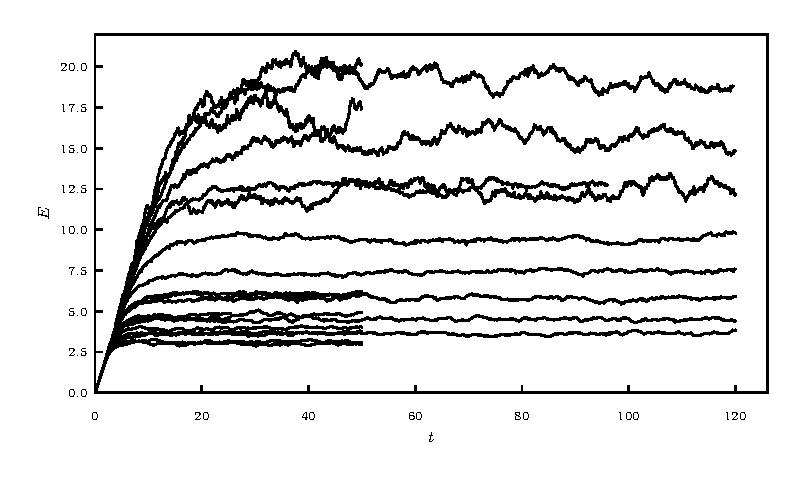
\includegraphics[]{paper_04_shallow_water/Pyfig/fig1}}
\caption{Space averaged energy, $E = E_K + E_A $, versus time for all
simulations. }
\label{fig_Evstime}
\end{figure}

\begin{figure}
\centerline{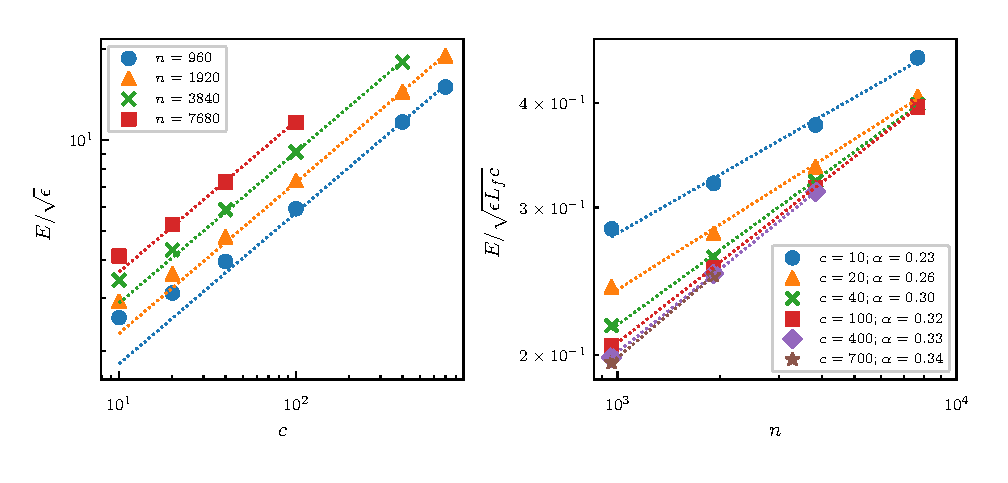
\includegraphics[]{paper_04_shallow_water/Pyfig/fig2}}
\caption{Left: Mean energy in the stationary state versus $ c $ for different
resolutions. The lines have slope $ 0.5 $, corresponding to $ E \propto c^{1/2}
$. Right: Normalised mean energy in the stationary state versus resolution $ n
$ for different $ c $.}
\label{MeanE}
\end{figure}



The time evolution of mean energy is shown in figure~\ref{fig_Evstime} for all
twenty simulations. After an initial period of growth, mean energy is levelling
out at different values for different runs. This is not the same picture as we
see in simulations of three-dimensional incompressible turbulence or stratified
turbulence, where all curves would have levelled out more or less at the same
value. We find that mean energy in the stationary state is a function of both $
c $ (or the Froude number) and resolution $ n $ and that the functional
dependence can be approximately written as
\begin{equation} \label{MeanEnergy}
E \sim \sqrt{\epsilon L_f c } \, n^{\alpha}  \, .
\end{equation}
 In figure~\ref{MeanE} to the
left, we see $ E/\sqrt{\epsilon} $ as a function of $ c $ for different resolutions $
n $. For each resolution the points are approaching a power law $ C_n c^{1/2} $
with increasing values of $ C_n $ for increasing $ n $. In the same figure to
the right we see $ E/\sqrt{\epsilon L_f c } $ for different values of $ c $. For
each $ c $ the points follow a power law $ n^{\alpha} $, where $ \alpha $ is
becoming slightly larger with increasing $ c $, approaching almost the same
value $ \alpha \approx 0.33 $ for the three highest values of $ c $. The
relation (\ref{MeanEnergy}) can be reformulated as
\begin{equation} \label{Dissipation}
\frac{\epsilon} {(E^{3/2} / L_f)} \sim \frac{E^{1/2}}{c} n^{-2\alpha} \, .
\end{equation}
Since the simulations are well resolved the dependence on resolution should not
be interpreted as consequence of the numerics but rather as a Reynolds number
effect, although it is not hundred per cent clear how a Reynolds number should
be defined in our case. We may note, however, that $ n \sim L_f/\delta x $ and in the case of Navier-Stokes viscosity
 we should have $ \delta x \propto \nu $, according to (\ref{Width}). Therefore,  $ n $ may be substituted by a Reynolds number. The normalised energy dissipation on the left-hand side of
(\ref{Dissipation}) will thus go to zero in the limit of large Reynolds number.
This is very different from three-dimensional turbulence where there is a local
Richardson-Kolmogorov cascade, in which energy is successively transferred from
large to small scales of motion. That the cascade is local means that eddies of
a particular scale are not directly influenced by eddies of widely different
scales. As a consequence, the normalised dissipation is of the order of unity
independent of Reynolds number \cite[]{Pope, TennekesLumley}. A review of the
experimental evidence and theoretical implications of this fundamental law of
Kolmogorov turbulence is given by \cite{Vassilicos2015}. Our result
(\ref{Dissipation}) suggests that SW wave turbulence does not fit into the
paradigm of a local Richardson-Kolmogorov cascade. Moreover, it is not only in
the limit of large Reynolds numbers the normalised dissipation will go to zero
but also in the limit of strong stratification, $ E^{1/2}/c \rightarrow 0 $.
This is different from three-dimensional stratified turbulence where the ratio
on the left-hand side of (\ref{Dissipation}) is of the order of unity in the
limit of strong stratification \cite[]{Lindborg2006, Brethouwer2007}.

That the energy transfer is not local in a system where the agent of dissipation is wave breaking or shock formation may be expected. According to the theory of ocean waves by  \cite{Phillips},
`wave interactions are usually incapable of transferring energy from a given wavenumber
band as rapidly as it is supplied by the wind'. Instead, energy is fed into each wave mode by the
wind field and sucked out from the same mode in `intermittent patches of foaming'
or `white horses'.  This may be a too simplified picture of SW water turbulence, since a broad band energy spectrum develops between the forcing and the dissipation wavenumbers.
Nevertheless,  shock formation suggests that there is a considerable direct energy transfer from large to very small wavelengths, without any intermediate steps.


The `four-fifths law' for the third-order structure function of Kolmogorov
turbulence is often derived using the assumption of a local cascade
\cite[]{Vassilicos2015} or the assumption that dissipation stays finite in the
limit of large Reynolds number \cite[]{Frisch}. As we just discussed, these
assumptions seem to be violated in the case of SW wave turbulence.
Nevertheless, the analogous law (\ref{eq_Kolmo}) is satisfied with a high degree of accuracy in our simulations. In
figure~\ref{Flux} we see the spectral energy flux from run W7 to the left and
the third-order structure function to the right. There is a broad constant flux
range with equipartition between KE and APE flux and an almost equally broad
range where (\ref{eq_Kolmo}) is satisfied, with equipartition between the two
third-order structure functions associated with KE and APE. The assumptions of
a local cascade and finite dissipation do not seem to be necessary in order for
the third-order structure function law (\ref{eq_Kolmo}) to be valid.



\begin{figure}
\centerline{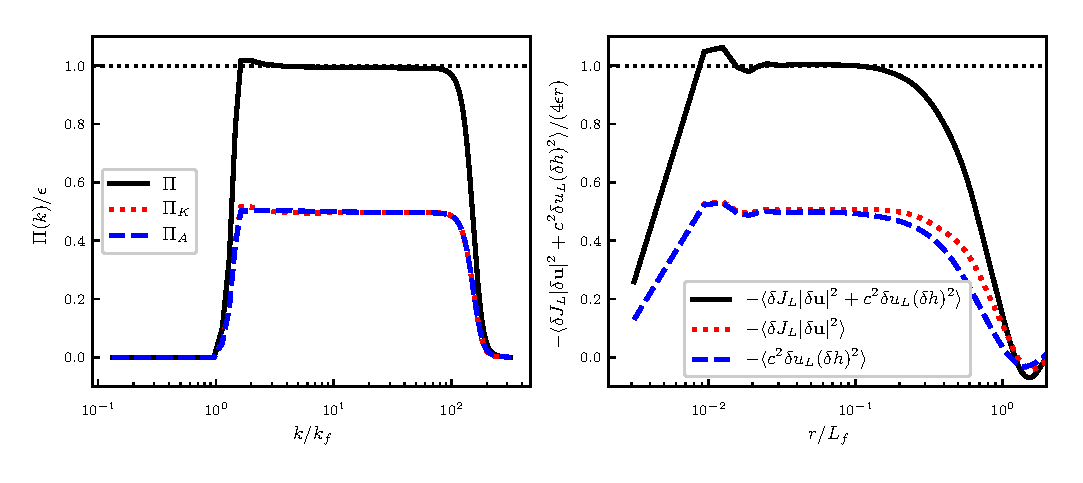
\includegraphics[]{paper_04_shallow_water/Pyfig/fig3}}
\caption{Left: Time averaged normalised spectral energy fluxes versus $ k/k_f
$. Right: Time averaged normalised third-order structure functions versus $
r/L_f $. From run W7. }
\label{Flux}
\end{figure}


\begin{figure}
\centerline{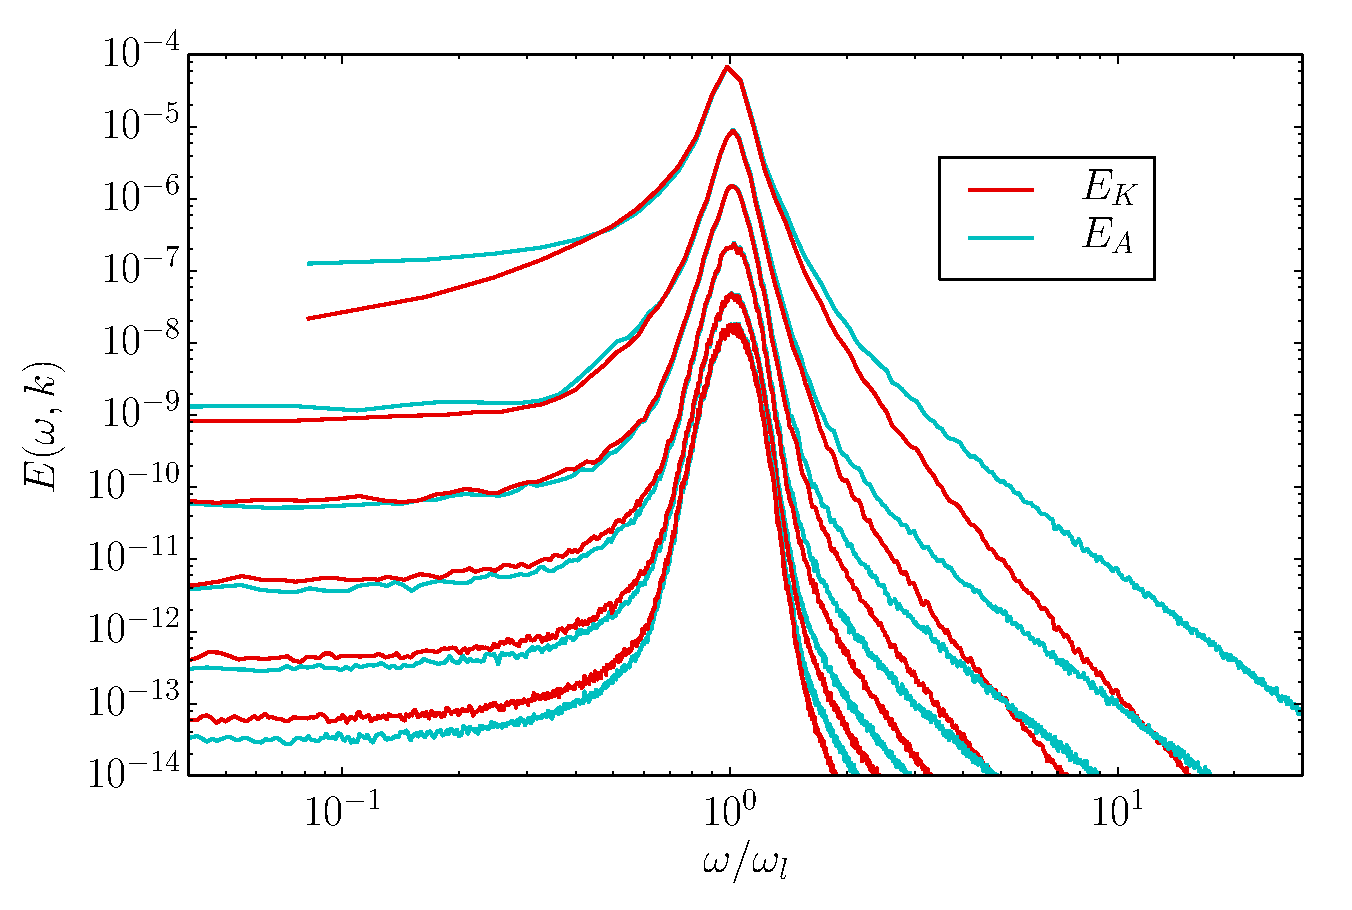
\includegraphics[width=3in]{paper_04_shallow_water/Pyfig/fig4}}
\caption{Frequency spectra of KE and APE for different $ k = \mid {\bf k} \mid
$, from run W7. The spectra are plotted as functions of $\omega/\omega_l$,
where $\omega_l = c k$. From top to bottom: $ k /\delta k = 12$, 27, 62, 143,
327, and 746. }
\label{fig_spatiotemp_spectra}
\end{figure}

\begin{figure}
\centerline{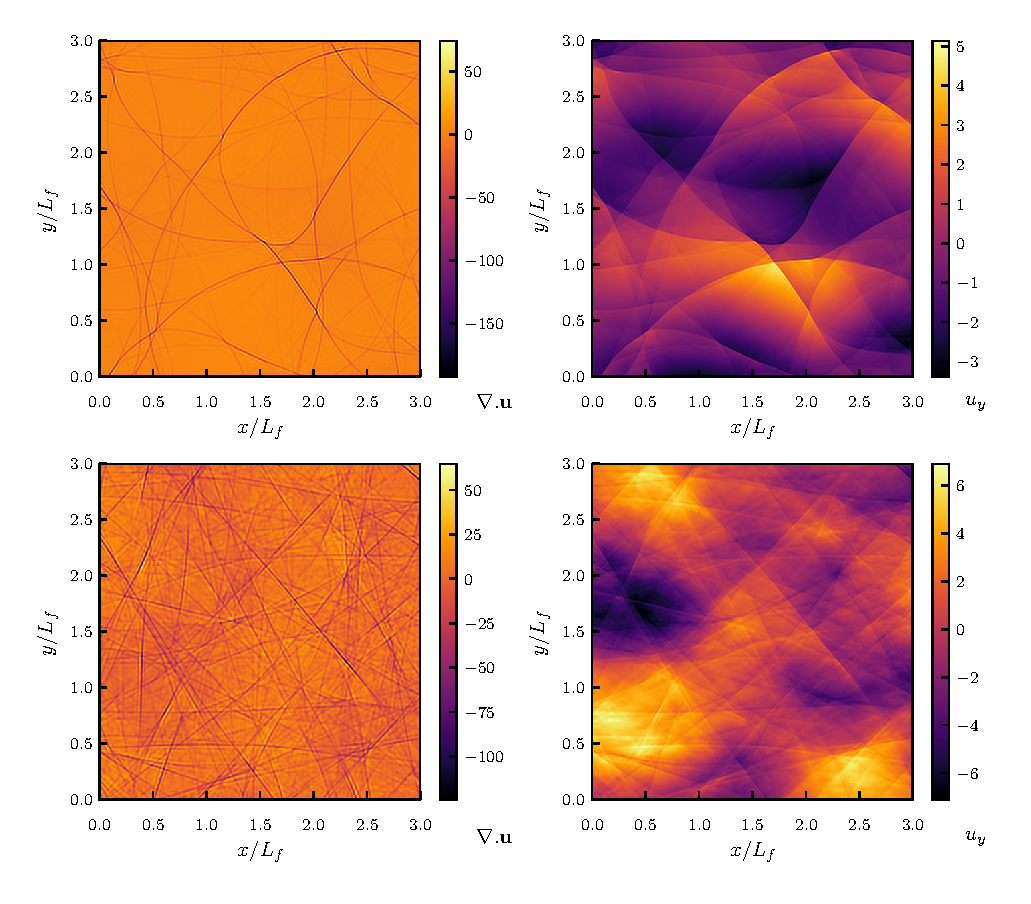
\includegraphics[]{paper_04_shallow_water/Pyfig/fig5}}
\caption{$(a,c)$ Divergence $ \bnabla \cdot {\bf u} $.  $(b,d)$ Velocity
component in the $ y $-direction: $ u_y $. $(a,b)$ Run W6. $(c, d)$ Run W17.
}
\label{Physical}
\end{figure}

\begin{figure}
\centerline{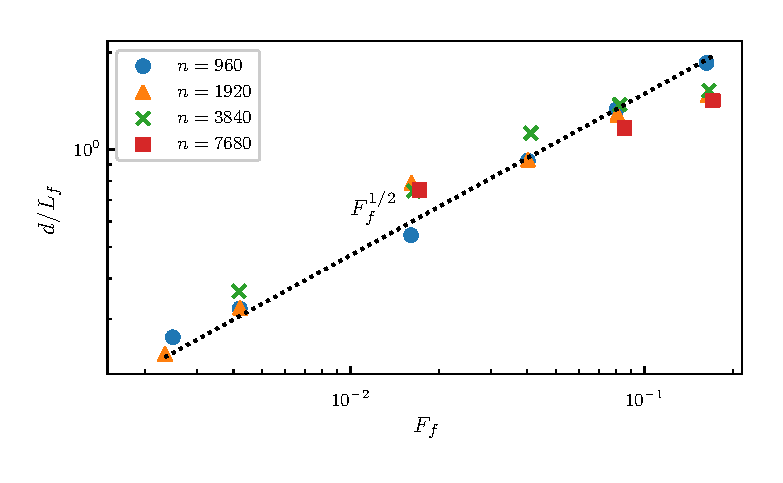
\includegraphics[width=9cm]{paper_04_shallow_water/Pyfig/fig6}}
\caption{Mean distance between the shocks as function of Froude number.  }
\label{fig_distance}
\end{figure}




The equipartition of the KE and APE spectral fluxes suggests that the flow to
leading order may be described as a collection of linear gravity waves with energy
equipartition in each mode. To investigate this further we have
collected time series of the flow variables from Fourier modes whose magnitudes
fall within certain shells, $ |{\bf k}| \in [ k -\delta k/2, \; k+
\delta k/2] $, and computed temporal power law spectra from these time series
and averaged over all wavenumbers in each shell. In other words, we have
computed KE and APE frequency spectra corresponding to different magnitudes of
modes. Figure~\ref{fig_spatiotemp_spectra} presents such spectra plotted as
functions of the normalised frequency $\omega/\omega_l$, where $ \omega_l = ck
$ is the linear wave frequency. The spectra are strongly dominated by peaks at
$\omega = \omega_l$. As can be seen, there is equipartition between KE and APE
in each shell. Although the widening of the peaks around the linear frequency
most likely is an effect of nonlinearities, we can quite safely conclude that
the time evolution of the flow variables in each Fourier mode to leading order
can be described as a linear wave.

Visualisations of the flow field give a completely different picture from what
may be expected from a collection of linear gravity waves. They are totally
dominated by the appearance of shock waves. In figure~\ref{Physical} we see
the divergence, $ \nabla \cdot {\bf u} $, to the left and the velocity
component in the $ y $-direction, $ u_y $, to the right.  Note that the total
area of the computational domain is sixteen times larger than the area of the
outcuts shown in the figures, since the side of the figures is $ 3 L_f
$, while the side of the computational domain is $ 12 L_f $.
The two figures at the
top are from run W6 while the two figures at the bottom are from run W17. The
difference between the two runs is that $ c $ is larger by a factor of $ 20 $
in W17 as compared to W6. To the left we see the shocks displayed as elongated
bands of negative divergence. That the divergence is negative at the shocks can
be understood from the fact that the velocity component perpendicular to the
shock always has a negative jump in the direction of shock propagation.
Apparently, the mean distance between the shocks is considerably smaller in run
W17 with the larger value of $ c $ compared to run $ W6 $ with the smaller
value of $ c $.
The shocks are also visible in the figures to right where $ u_y
$ is displayed. It may be interesting to note that the shocks along the $ x
$-axis appear as extra sharp in this plot, since there is a strong jump of $
u_{y} $ over these shocks, while the shocks along the $ y $-axis are hardly
visible, since there is no jump of $ u_{y} $ over these. In the two figures to
the right we see a variation of the flow field over the length scale $ L_f $
which is not seen in the two figures to the left. This variation is evidently a
footprint of the random forcing. Although the forcing length scale $ L_f $ is
the same in the two simulations the mean distance, $ d $, between the shocks is
much smaller in run $ W17 $ than in run $ W6 $, which may come as a surprise. Another interesting observation is that the shocks in run W17 (lower figures) appear to have smaller curvature on average than the shocks in run W6 (upper figures). In both runs, the shocks are weak in the sense that the Mach number is close to unity and the interaction between the shocks should therefore be weak \cite[see][]{ApazidisEliasson2018}. However, as measured by the Mach number  (\ref{Mach}), the shocks are much weaker in run W17, where $ c $ is larger by a factor of 20 as compared to run W6 and $ d $ also is smaller. The shock interaction should therefore be weaker in run W17, which may explain the observation that the curvature of the shocks is smaller in run W17 than in run W6.
We have calculated  the mean distance, $ d $, between the shocks by counting the number of negative spikes
of the divergence along two hundred lines parallel to the $ x $-axis and equally many
parallel to the $ y $-axis and then divided total length of all the lines by
the number of spikes. Generally, we found that $ d \propto c^{-1/2} $, or
\begin{equation} \label{MeanDistance}
d \sim L_f F_f ^{1/2} \, ,
\end{equation}
independent of resolution $ n $. In figure~\ref{fig_distance} we have plotted
$ d/L_f $ versus Froude number for all twenty runs. As can be seen, the points
follow the $ F_f^{1/2} $-curve quite well, although there seems to be a slight
systematic deviation at the highest $ F_f $.

\begin{figure}[htp!]
\centerline{
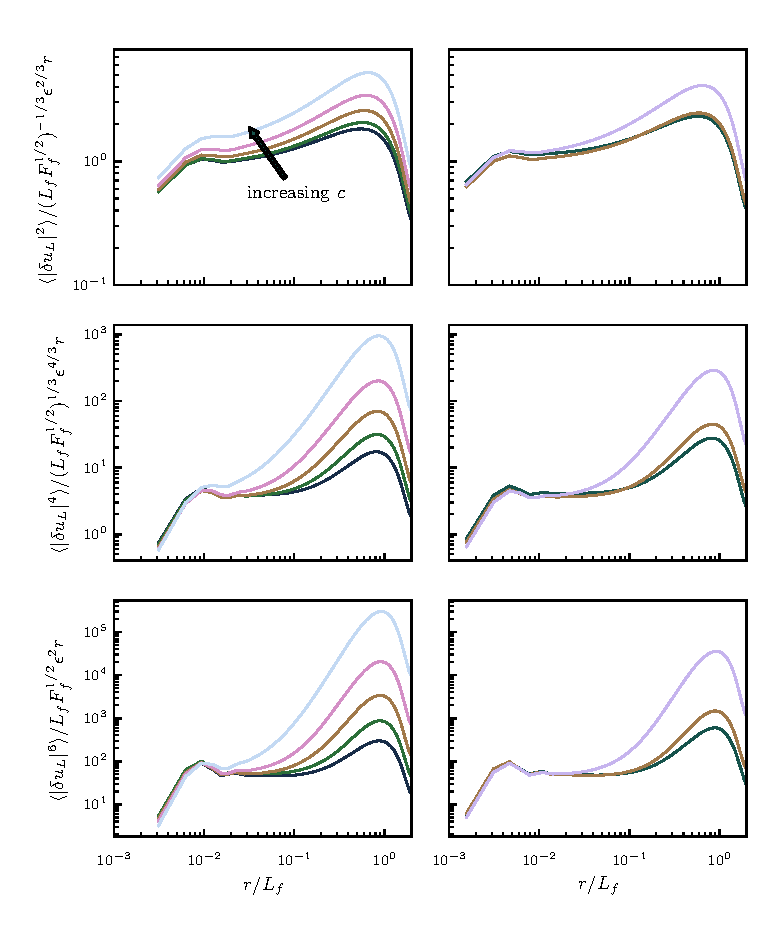
\includegraphics[]{paper_04_shallow_water/Pyfig/fig7}}
\caption{From top to bottom: second-, fourth- and sixth-order compensated and
    normalised longitudinal structure functions. $(a,c,e)$ Runs with $ n=3840 $: W3,
W7, W11, W14 and W18. $(b,d,f)$ Runs with $ n = 7860 $: W4, W8 and W15. }
\label{fig_StrucFunc}
\end{figure}

\begin{figure}
\centerline{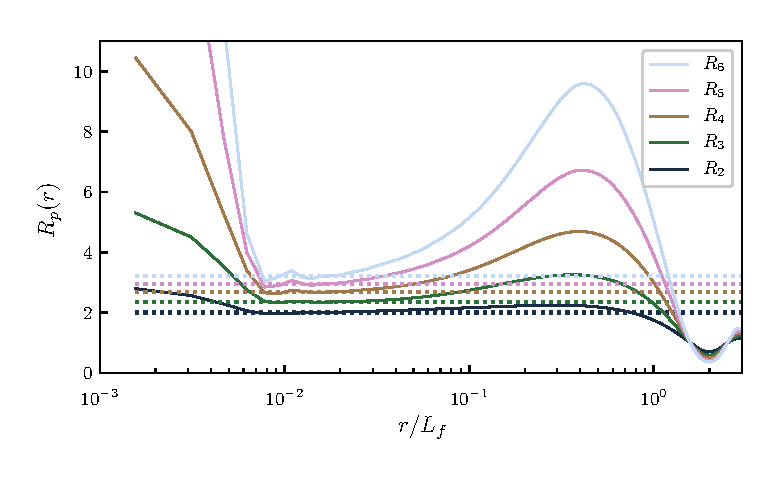
\includegraphics[width=11cm]{paper_04_shallow_water/Pyfig/fig8}}
\caption{
Ratio of the structure functions
$R_p(r) = \mean{|\delta u_L|^p} / \mean{|\delta u_T|^p}$ from run W8,
for $ p = 2, \, 3, \, 4, \, 5, \, 6. $
The dotted straight lines indicate the values predicted by (\ref{Ratio}):
$R_2 = 2$, $R_3 = 3\pi/4$,  $R_4 = 8/3$, $ R_5 = 15 \pi /16 $ and $ R_6 = 16/5 $.}
\label{fig_ratio}
\end{figure}

\begin{figure}
\centerline{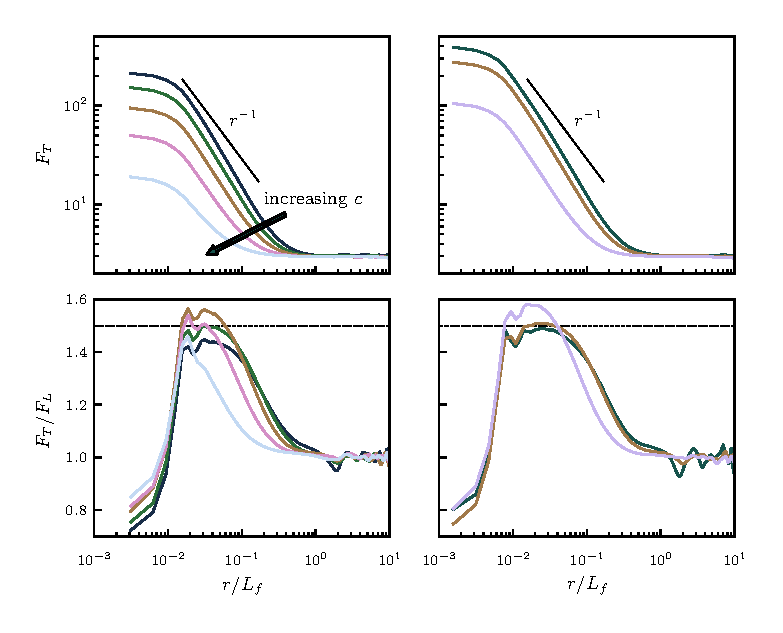
\includegraphics[]{paper_04_shallow_water/Pyfig/fig9}}
\caption{ Top: Flatness factor of transverse velocity increments. Bottom: Ratio between transverse and longitudinal flatness factor. Left: runs with $ n=3840 $: W3,
W7, W11,  W14 and W18. Right: runs with $ n = 7860 $: W4, W8 and W15.  The dotted straight lines indicate the value 1.5 predicted by the shock model.  }
\label{fig_flatness}
\end{figure}

\begin{figure}
\centerline{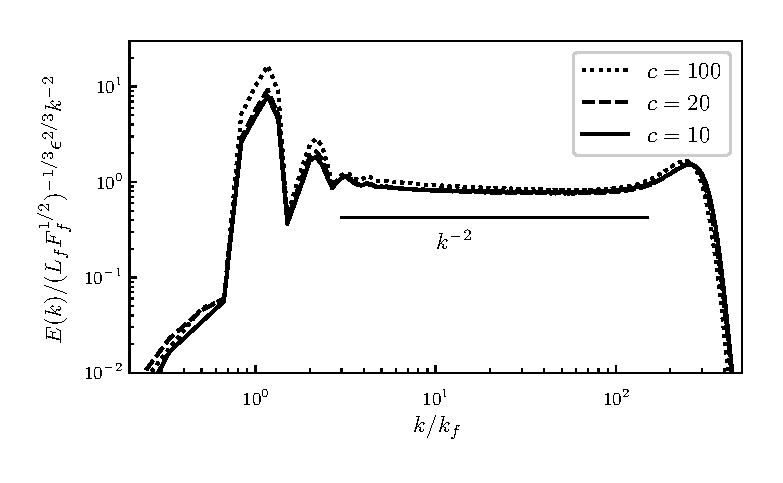
\includegraphics[]{paper_04_shallow_water/Pyfig/fig10}}
\caption{Time averaged compensated and normalised energy spectra
from runs with $ n = 7680 $: W4, W8 and W15.}
\label{fig_spectra_c40}
\end{figure}

\begin{figure}
\centerline{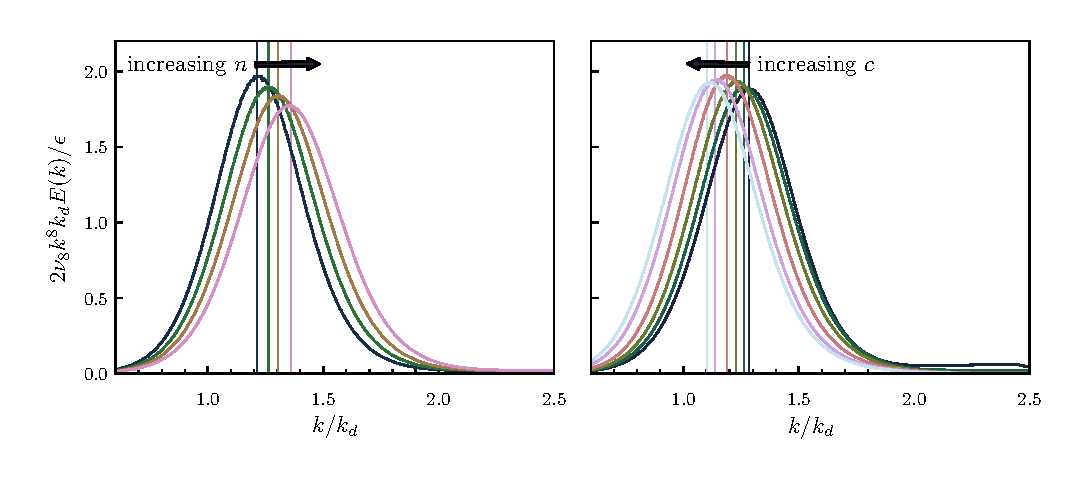
\includegraphics[]{paper_04_shallow_water/Pyfig/fig11}}
\caption{Time averaged normalised dissipation spectra. Left: Constant $ c = 20 $ and varying $ n $, runs  W5, W6, W7 and W8. Right: Constant $ n= 1920 $ and varying $ c $, runs W2, W6, W10, W13, W17 and W20. The vertical lines indicate the wavenumbers of the maxima.}
\label{fig_disspectra}
\end{figure}



We will now present the results for the structure functions. Substituting
(\ref{MeanDistance}) into (\ref{StrucFunc}) we find that the structure
functions are expected to scale as
\begin{equation} \label{StrucFunc2}
\meane{|\delta u |^p}  \sim \meane{(c|\delta h |)^p} \sim  (L_f F_f^{1/2})^{p/3-1}  \epsilon^{p/3}  r  \, .
\end{equation}
for separation distances that fulfil the condition $ \delta x \ll r \ll d $.
The scaling (\ref{StrucFunc2}) is
expected to become better and better fulfilled with decreasing $ c $ (or
increasing $ F_f $). According to (\ref{MeanDistance})
$ d $ is increasing with $ F_f $, and the scaling range is therefore becoming
wider for decreasing $ c $, if $ \delta x $ or the resolution  is kept
constant. The scaling
(\ref{StrucFunc2}) is also expected to become better and better fulfilled with
increased resolution $ n $, since $ \delta x $ is decreasing with increasing $
n $.

As expected, we have found that the displacement structure functions scale
exactly in the same way as the velocity structure functions, and for this reason we only plot
velocity structure functions. In figure~\ref{fig_StrucFunc} we see the
compensated and normalised second-, fourth- and sixth-order longitudinal
structure functions from the five simulations with $ n = 3840 $ to the left and
the three simulations with $ n = 7860 $ to the right. At small separation, $ r
< \delta x $, the structure functions have the dependence $ \sim r^{p} $, which
is characteristic of a smooth velocity field, indicating that the shocks are
reasonably well resolved. There is a small bump around the shock width, $ r
\approx \delta x $, and at $ r > \delta x $, there is a range where the
compensated structure functions are flat, or almost flat. As expected, this
range is becoming broader for smaller $ c $ (or larger $ F_f $). The range is
also broader in the higher resolution runs to the right as compared to the
lower resolution simulations to the left. There is clearly a better collapse of
the curves for the sixth-order structure functions compared to the second-order
structure functions. This is not surprising, since the shock contribution to
the structure functions should become increasingly dominant with increasing
order. Plots of the transverse structure functions are very similar to the
plots of the longitudinal structure functions, with the difference that the
transverse structure functions are somewhat smoother at $ r \approx \delta x $.
In figure~\ref{fig_ratio} we see the ratio $ R_{p}(r) = \langle \mid \delta
u_L \mid ^{p} \rangle / \langle \mid \delta u_T \mid ^{p} \rangle$ for $ p=
2,3,4,5,6 $ from run W8, together with dotted straight lines, indicating the
values predicted by (\ref{Ratio}). As can be seen, there is a quite good
agreement with the predicted values in a limited range of separations, $ r >
\delta x $. Somewhat unexpectedly, the range in which there is a good agreement
becomes more narrow with increasing $ p $, an observation that we cannot
explain. It may also be noted that $ R_2 \rightarrow 3 $ in the limit of small
$ r $, which is the theoretical single point limit for an irrotational
isotropic field. In figure~\ref{fig_flatness} we see the flatness factor, $
F_T $, of the transverse structure functions at the top and the ratio, $
F_T/F_L $, at the bottom. The figures to the left show the results from the
five simulations with $ n = 3840 $ and the figures to the right show the
results from the three simulations with $ n = 7860 $. The flatness factor shows
increasingly large values for decreasing $ r $ with a dependence that is rather
close to but somewhat steeper than $ r^{-1} $. At small $ r $ the curves are
levelling out at very large values. For $ n = 7869 $ and $ c = 10 $ we see that
$ F_{T} \approx 400 $ at small $ r $. The degree to which the flatness factor
is increasing with decreasing scale is by some authors defined as the most
appropriate measure of spatial intermittency \cite[see for example][]{Frisch}.
If this measure is used, SW wave turbulence is, indeed, extremely intermittent.
In the two figures at the bottom we see that $ F_{T}/F_{L} \approx 1.5 $ in a
limited range of separations, $ r > \delta x $, which is becoming somewhat
broader as $ c $ is increasing and is also somewhat broader in the higher
resolution runs shown to the right as compared to the lower resolution runs
shown to the left. This is in accordance with the shock model predictions
(\ref{FL}) and (\ref{FT}).

Finally, we present energy and dissipation spectra. As expected, we found that APE and KE
spectra were almost identical, and therefore, we only plot the
total spectra. In figure~\ref{fig_spectra_c40} we see  compensated and
normalised energy spectra from the three highest resolution runs. The
compensated spectra are almost flat in a broad range. At the high wavenumber
end the compensated spectra show a `bottleneck', which we interpret as a
signature of the shocks. The $ k^{-2} $-dependence and the associated scaling predicted
by (\ref{Spectra}) are very well satisfied in a limited range of high wavenumbers close to the bottleneck. At smaller wavenumbers the spectra are
becoming somewhat steeper than $ k^{-2} $ and the spectrum from the run with
largest $ c $ does not collapse perfectly onto the other two spectra.  In figure \ref{fig_disspectra}
 we see normalised dissipation spectra for fixed $ c= 20 $ and different $ n $ to the left, and fixed $ n = 1920 $
and different $ c $ to the right. First we note that the spectra go to zero quite nicely for large $ k $, indicating that the shock width $ \delta x $ is well resolved. Second, we note that there is a slight shift of the maximum in both figures, even though we have normalised the wavenumber by $ k_d = 1/\eta_8 $.   These shifts may be explained by the estimate (\ref{EtaEight}) predicting that $ \delta x $ should vary slightly with $ d $. If the maximum of the dissipation spectra is associated with $ \delta x $, there should be a shift of the maximum  to the right with increasing $ n $ and to the left with increasing $ c $, since $ d \propto c^{-1/2} $.
 The ratio between the maximum and the minimum $ n $ in the left figure is equal to 8 and  according to (\ref{EtaEight}) the corresponding ratio between the wavenumbers at which the maxima are observed should be $ 8^{1/21} \approx 1.1 $, which is exactly the value we observe. The ratio between the maximum and minimum $ c $ in the right figure is equal to $ 70 $. Assuming that $ d \propto c^{-1/2} $ the ratio between the wavenumbers at which the maxima are observed should be $ 70^{1/42} \approx 1.1 $, while the observed ratio is equal to $ 1.16 $. In the latter case, there is no exact quantitative agreement between the predicted trend and the numerical results.




\section{Conclusions and discussion}

We have carried out a theoretical and numerical investigation of SW wave
turbulence. First, we derived the SW analogue (\ref{eq_Kolmo}) of the
`four-fifths' law of Kolmogorov turbulence. Using this relation and
straightforward statistical and geometrical arguments we developed a simple
shock model predicting that the shock amplitude scales as $ (\epsilon d)^{1/3}
$, where $ d $ is the mean distance between the shocks, and that the
$ p $th-order structure function above a certain minimum will scale as
$ (\epsilon d)^{p/3} r/d $. Then, we carried out a series of forced-dissipative
simulations, varying the Froude number and the resolution. In all simulations,
a statistically stationary state was reached and in all simulations we
observed shocks. The flow variables in each Fourier mode were found to evolve
in accordance with linear wave dynamics, with equipartition between APE and KE
over a period. The third-order structure function relation was fulfilled with a
high degree of accuracy. From the simulations we made two interesting
observations that fall outside the predictive scope of the model. The first
observation was that mean energy in the stationary state approximately scales
as (\ref{MeanEnergy}), suggesting that the normalised dissipation
(\ref{Dissipation}) will go to zero both in the limit of small viscosity and
large wave speed. A similar observation was made when we used a second-order diffusion operator instead of hyper diffusion (see Appendix A).
This is different from three-dimensional Kolmogorov
turbulence as well as strongly stratified turbulence, where, in both cases,
dissipation is finite in the limit of small viscosity, and in the latter case
also is independent of the degree of stratification. This observation suggests
that SW wave turbulence does not fit into the paradigm of a local
Richardson-Kolmogorov cascade.  It remains a theoretical challenge to give a quantitative explanation of the growth of energy with increased Reynolds number.
As far as we can see, such an explanation would require a completely novel theoretical development.
The second observation we made was that the mean
distance between the shocks scales as $ c^{-1/2} $, if the other parameters are
held constant. As we increased $ c $, the shocks were thus becoming denser.
Using this observation we tested the shock model by plotting the normalised and
compensated structure functions of different orders. Generally we found that
there was a quite good agreement between the simulation results and the model
predictions, becoming better with decreasing wave speed and increasing
resolution.

Combining the model and the observations we can get a quite good picture of the
dynamics in the limit of weak nonlinearities, $ F_{f} \rightarrow 0 $. The
picture may become more vivid if we say `wave breaking' where we previously have
talked about shock formation, and also say `wavelengths' were we previously
have talked about length scales. We identify the longest wavelength, $
\lambda_l $, with the forcing scale $ L_f $ and the breaking wavelength, $
\lambda_b $, with the mean distance, $ d $, between the shocks. There are two
dynamically different regimes, the short wave regime, $ [\delta x, \;
\lambda_b] $, and the long wave regime, $ [\lambda_b, \, \lambda_l] $. We first
consider the latter, whose width scales $ \lambda_{l} /\lambda_b \sim
F_f^{-1/2} $. Identifying the amplitude of the breaking waves with the shock
amplitude, $ (\epsilon d)^{1/3} $, we find that the ratio between the amplitude of
the longest waves and the breaking waves scales as $ E^{1/2}/(\epsilon d)^{1/3}
\sim F_{f}^{-5/12} n^{\alpha/2} $, where we may substitute $ n $ with a
Reynolds number. Thus, for small $ F_f $ and large Reynolds
numbers the longest waves are not directly influenced by wave breaking. The
Reynolds number dependence of the amplitude ratio makes it unlikely that a
general similarity theory can be easily formulated for this range. Therefore,
predictions from weak turbulence theory \cite[for
example][]{ZakharovSagdeev1970} are not likely to hold for this range, although
it is not directly influenced by wave breaking. The exact values of the power
law exponents in the argument leading to this conclusion are, of course, not
important. As for the short wave regime, the width scales as $ \lambda_b
/\delta x \sim F_f^{1/2} $ for fixed $ \delta x $ or fixed Reynolds number. As
$ F_{f} \rightarrow 0 $ the range will eventually become so narrow so that
breaking will disappear. As argued in Appendix A, the condition $ \lambda_b \gg \delta x $ leads to a wave breaking condition involving both the Reynolds number,  $ Re  \equiv \epsilon^{1/3} L_f^{4/3} /  \nu $, and  the Froude number. If $ \lambda_b \propto F_f^{m} $ we obtain the condition $ Re F_f^{4m/3} \gg 1 $ and in the special case when $ m = 1/2 $, the condition is
\begin{equation} \label{WC}
Re F_f^{2/3} \gg 1 \, .
\end{equation}
Thus,  for a given Reynolds number, no matter how large, wave breaking will be absent provided that $ F_f $ is sufficiently small. On the other hand, if (\ref{WC}) not only is a necessary but also a sufficient condition,  wave breaking will be present for any given $ F_f $, no matter how small, provided that $ Re $ is sufficiently large. The condition (\ref{WC}) is analogous to the condition for the presence of turbulence in a stratified fluid, also involving both the Reynolds number and a Froude number \cite[]{Brethouwer2007}. The horizontal and vertical length scales of stratified turbulence scale as $ l_h \sim u^{3}/\epsilon $ and $ l_v \sim u/N $, respectively, where $ u $ is a characteristic horizontal velocity and $ N $ is the Brunt-V\"ais\"al\"a frequency. As stratification becomes stronger ($ N $ is increasing), $ l_v $ is becoming smaller.  However, in order for turbulence to be present $ l_v $ must be much larger than the Kolmogorov scale, $ \nu^{3/4}/\epsilon^{1/4} $, which leads to the condition $ Re F_h^2 \gg 1 $, where $ F_h = u/(l_h N) $ is a Froude number based on the horizontal length scale.

 The present study makes some advancement of the understanding of compressible turbulence. Previously, energy flux relations  have
 been derived  for a compressible and barotropic fluid by \cite{Falkovich2010} and \cite{Galtier2011}.  Unlike (\ref{FluxT}) these flux relations are not exclusively expressed in terms of third-order structure functions, {\em i. e.} third-order moments of increments of flow variables.
As is clear from our analysis, in the general case of a compressible and irrotational fluid the KE flux can be expressed in this way.  It seems to be more of a specific property that the APE flux also can be expressed in terms of a third-order structure function, a property that the SW system shares with the Boussinesq system with constant Brunt-V\"ais\"al\"a frequency, in which case APE also is quadratic in buoyancy \cite[]{Augier2012}.
In this context,  a comparison between our analysis and the analysis  by
\cite{Galtier2011} of  isothermal compressible turbulence  is revealing. In the
latter case, the pressure is linear in density, $ p = c_t^2 \rho $, where $ c_t
$ is the isothermal speed of sound, and the internal energy per unit volume is
equal to $ c_t^2 \rho \ln (\rho/ \rho_0) $, where $ \rho_0 $ is an ambient
reference density. Due to this  logarithmic dependence, the internal energy
flux is not expressible in terms of a structure function. However, an equation
system which is equivalent to the SW equations can be obtained by replacing the
pressure term, $ \rho^{-1} \nabla p = \rho^{-1} c_t^{2} \nabla \rho $, in the
isothermal momentum equation, by $ \rho_{0}^{-1} c_t^{2} \nabla \rho $, which
may be motivated if density fluctuations are small. The expression for the
internal energy per unit volume of the modified system is  $ c_t^2
\rho^2/2\rho_{0} $, which is equivalent to the SW potential energy. (To see how the logarithmic and quadratic expressions for the internal energy are
 related, write $ \rho = \rho_0(1+\eta) $, expand in $ \eta $ and keep  terms up to second-order:
 $ c_t^2\rho \ln(\rho/\rho_0) \approx c_t^2 \rho_0(1+\eta)(\eta - \eta^2/2) \approx   c_t^2 \rho^2/2 \rho_0 - c_t^2 \rho_0/2 $.
 For small density fluctuations the two expressions only differ by a constant.) As a consequence of this quadratic dependence, the internal energy flux is expressible in terms of a structure function. It may be conjectured that the modified equation system is a good model for isothermal acoustic turbulence and that a flux relation which  equivalent to (\ref{FluxT}) also should hold for this case. In the three-dimensional case we then obtain
 \begin{equation}
\meane{ \delta (\rho u_L)    |\delta \uu|^2  }
+ c_t^2\meane{ \delta u_L(\delta \rho)^2  } /\rho_0 = - \frac{8}{3} \epsilon r \, ,\label{eq_Kolmo3}
\end{equation}
where  $ \epsilon $ here is the mean energy dissipation rate per unit volume.

While isothermal acoustic turbulence may have some interesting application for a radiating gas \cite[]{Stein1967}, standard text book acoustics is not isothermal but isentropic. The  condition of constant entropy puts us in a dilemma when we analyse an acoustic field as a forced-dissipative system, since dissipation inevitably is associated with entropy production.  According to arguments of \cite{KadomtsevPet1973}, an acoustic field is always dissipated by weak shocks if the Reynolds number is sufficiently large,  and this should be true in two as well as in three dimensions.  Given the numerical results of the present study such a hypothesis seems reasonable, since shock waves have similar stability properties
in two and three dimensions \cite[]{ApazidisEliasson2018, LivertsApazidis2016}.  The shock wave hypothesis offers an elegant way out of the isentropic dilemma, since it implies that entropy production is concentrated at the shocks, while the rest of the field can be treated as isentropic. In a companion paper \cite[]{Lindborg2019}, scaling relations for such an acoustic field are derived, using the weak shock relations and the entropy equation. It turns out that these scaling relations are analogous to the relations for shallow water wave turbulence, with the  difference
that the mean energy dissipation rate, $ \epsilon $, is replaced by $ \epsilon + \chi $, where $ \chi $ is a quantity associated with entropy production due to heat conduction. If  the Prandtl number is of the order of unity, $ \chi $ is of the same order as $ \epsilon $.  The shock amplitude scales as $ \Delta u \sim (\epsilon + \chi)^{1/3} d^{1/3} $, where $ d $ is the characteristic distance between the shocks and the third-order longitudinal structure function scales as $ \langle \delta u_L^{3} \rangle = -C (\epsilon + \chi)r $, where $ C $ is a constant of the order of unity, which can be determined exactly in the weak shock limit.

Acoustic turbulence is an example of a wave breaking system where the concepts and methods we have developed to analyse SW water turbulence can be applied in a fruitful way.  We believe that there may be other such examples.


\vskip 0.3 cm

\noindent The authors would like to thank Gregory Falkovich and Sergey Nazarenko for  fruitful criticism of an early version of the manuscript, Sebastien Galtier for making a check of the final manuscript and three anonymous reviewers for useful comments. Financial
support from the Swedish Research Council (VR) is gratefully
acknowledged. The simulations were performed
on resources provided by the Swedish National Infrastructure
for Computing (SNIC) at PDC.



\appendix

\section{Simulations with Laplacian diffusion}
%\label{app_comp}
On the request from the reviewers we have carried out a set of simulations using Laplacian diffusion, $ \nu \nabla^{2} $, to check that similar results are obtained in this case as when we use higher-order diffusion $ \nu_8 \nabla^{8} $.
A number of test simulations with resolution $ n = 960 $ and $ c= 10 $ were
first carried out using different values of the viscosity, until we determined a value which was sufficiently large for the shocks to be resolved, but not unnecessarily large.
This value was then used for all simulations with $ n = 960 $. For the more
highly resolved simulations the viscosity was then set as $ \nu \propto n^{-1} $, in accordance with the prediction  (\ref{Width}) for the shock width.
We define the Reynolds number as $ Re \equiv \epsilon^{1/3} L_f^{4/3}/\nu $, which is proportional to $ n $, since $ \nu \propto n^{-1} $.
The simulations are listed in table 2.


%TODO fix cite[] -> citep/parencite?




\begin{table}
\begin{center}

\begin{tabular}{lrrrrrrrrr}
\toprule
{} &   $n$ &  $c$ &  $\nu_2$ &  $\epsilon$ &  $\frac{k_d}{k_f}$ &   $F_f$ &  $Re$ &  $ReF_f^{2/3}$ &  $t_{\max}$ \\
\midrule
WL1  &   960 &   10 &   0.0985 &       0.998 &                    22.6 &   0.161 &  68.0 &           20.1 &          25 \\
WL2  &  1920 &   10 &   0.0492 &       0.985 &                    45.3 &   0.160 &   136 &           40.0 &          25 \\
WL3  &  2880 &   10 &   0.0328 &       0.984 &                    67.9 &   0.160 &   203 &           59.9 &          25 \\
WL4  &  3840 &   10 &   0.0246 &       0.993 &                    90.5 &   0.161 &   272 &           80.3 &          25 \\
WL5  &  7680 &   10 &   0.0123 &        1.00 &                     181 &   0.161 &   545 &            161 &          25 \\
WL6  &   960 &   20 &   0.0985 &       0.994 &                    22.6 &  0.0803 &  68.0 &           12.6 &          25 \\
WL7  &  2880 &   20 &   0.0328 &       0.982 &                    67.9 &  0.0800 &   203 &           37.7 &          25 \\
WL8  &  3840 &   20 &   0.0246 &       0.983 &                    90.5 &  0.0800 &   271 &           50.3 &          25 \\
WL9  &  7680 &   20 &   0.0123 &        1.00 &                     181 &  0.0805 &   545 &            102 &          25 \\
WL10 &   960 &   40 &   0.0985 &       0.985 &                    22.6 &  0.0400 &  67.7 &           7.93 &          25 \\
WL11 &  2880 &   40 &   0.0328 &       0.981 &                    67.9 &  0.0400 &   203 &           23.7 &          25 \\
WL12 &  3840 &   40 &   0.0246 &       0.978 &                    90.5 &  0.0399 &   270 &           31.6 &          25 \\
WL13 &  7680 &   40 &   0.0123 &       0.991 &                     181 &  0.0401 &   543 &           63.6 &          25 \\
WL14 &   960 &  100 &   0.0985 &       0.976 &                    22.6 &  0.0160 &  67.5 &           4.28 &          25 \\
WL15 &  2880 &  100 &   0.0328 &       0.961 &                    67.9 &  0.0159 &   202 &           12.7 &          25 \\
WL16 &  3840 &  100 &   0.0246 &       0.972 &                    90.5 &  0.0159 &   270 &           17.1 &          25 \\
WL17 &   960 &  200 &   0.0985 &       0.988 &                    22.6 & 0.00801 &  67.8 &           2.72 &          25 \\
WL18 &  2880 &  200 &   0.0328 &       0.928 &                    67.9 & 0.00785 &   199 &           7.87 &          25 \\
WL19 &  3840 &  200 &   0.0246 &       0.934 &                    90.5 & 0.00786 &   266 &           10.5 &          25 \\
\bottomrule
\end{tabular}


\label{Table2}



\caption{Parameters for all the simulations executed with laplacian viscosity.
$ n $: number of nodes in each direction, $ c $: wave speed, $ \nu  $:  viscosity, $ \epsilon $: time
averaged mean energy dissipation in the stationary state, $ k_{d}/ k_f $: ratio
between dissipation wavenumber and forcing wavenumber, $F_f $: Froude
number, $Re$: Reynolds number, $ t_{max} $: end time of simulation.}
\end{center}
\end{table}

\begin{figure}
\centerline{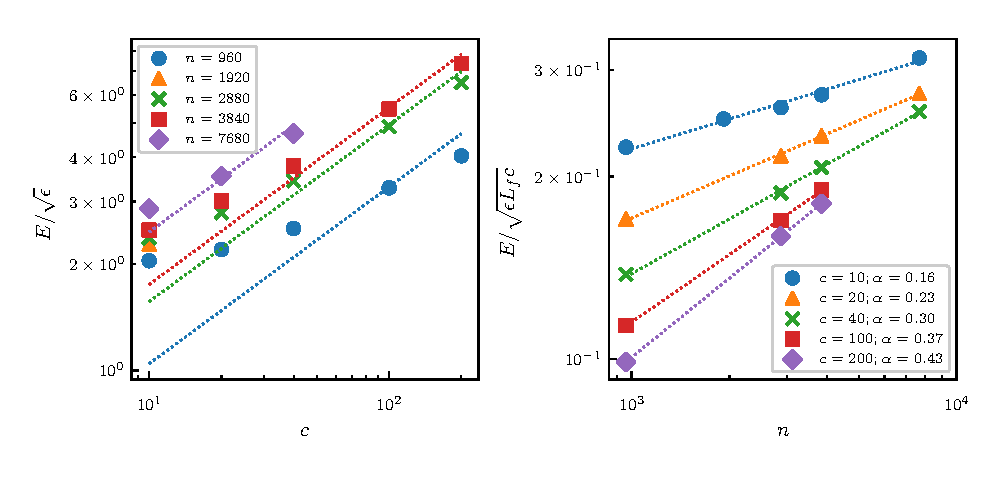
\includegraphics[]{paper_04_shallow_water/Pyfig/fig12}}
\caption{Left: Mean energy in the stationary state versus $ c $ for different
resolutions. The lines have slope $ 0.5 $, corresponding to $ E \propto c^{1/2}
$. Right: Normalised mean energy in the stationary state versus resolution $ n
$ for different $ c $.}
\label{MeanE2}
\end{figure}

\begin{figure}
\centerline{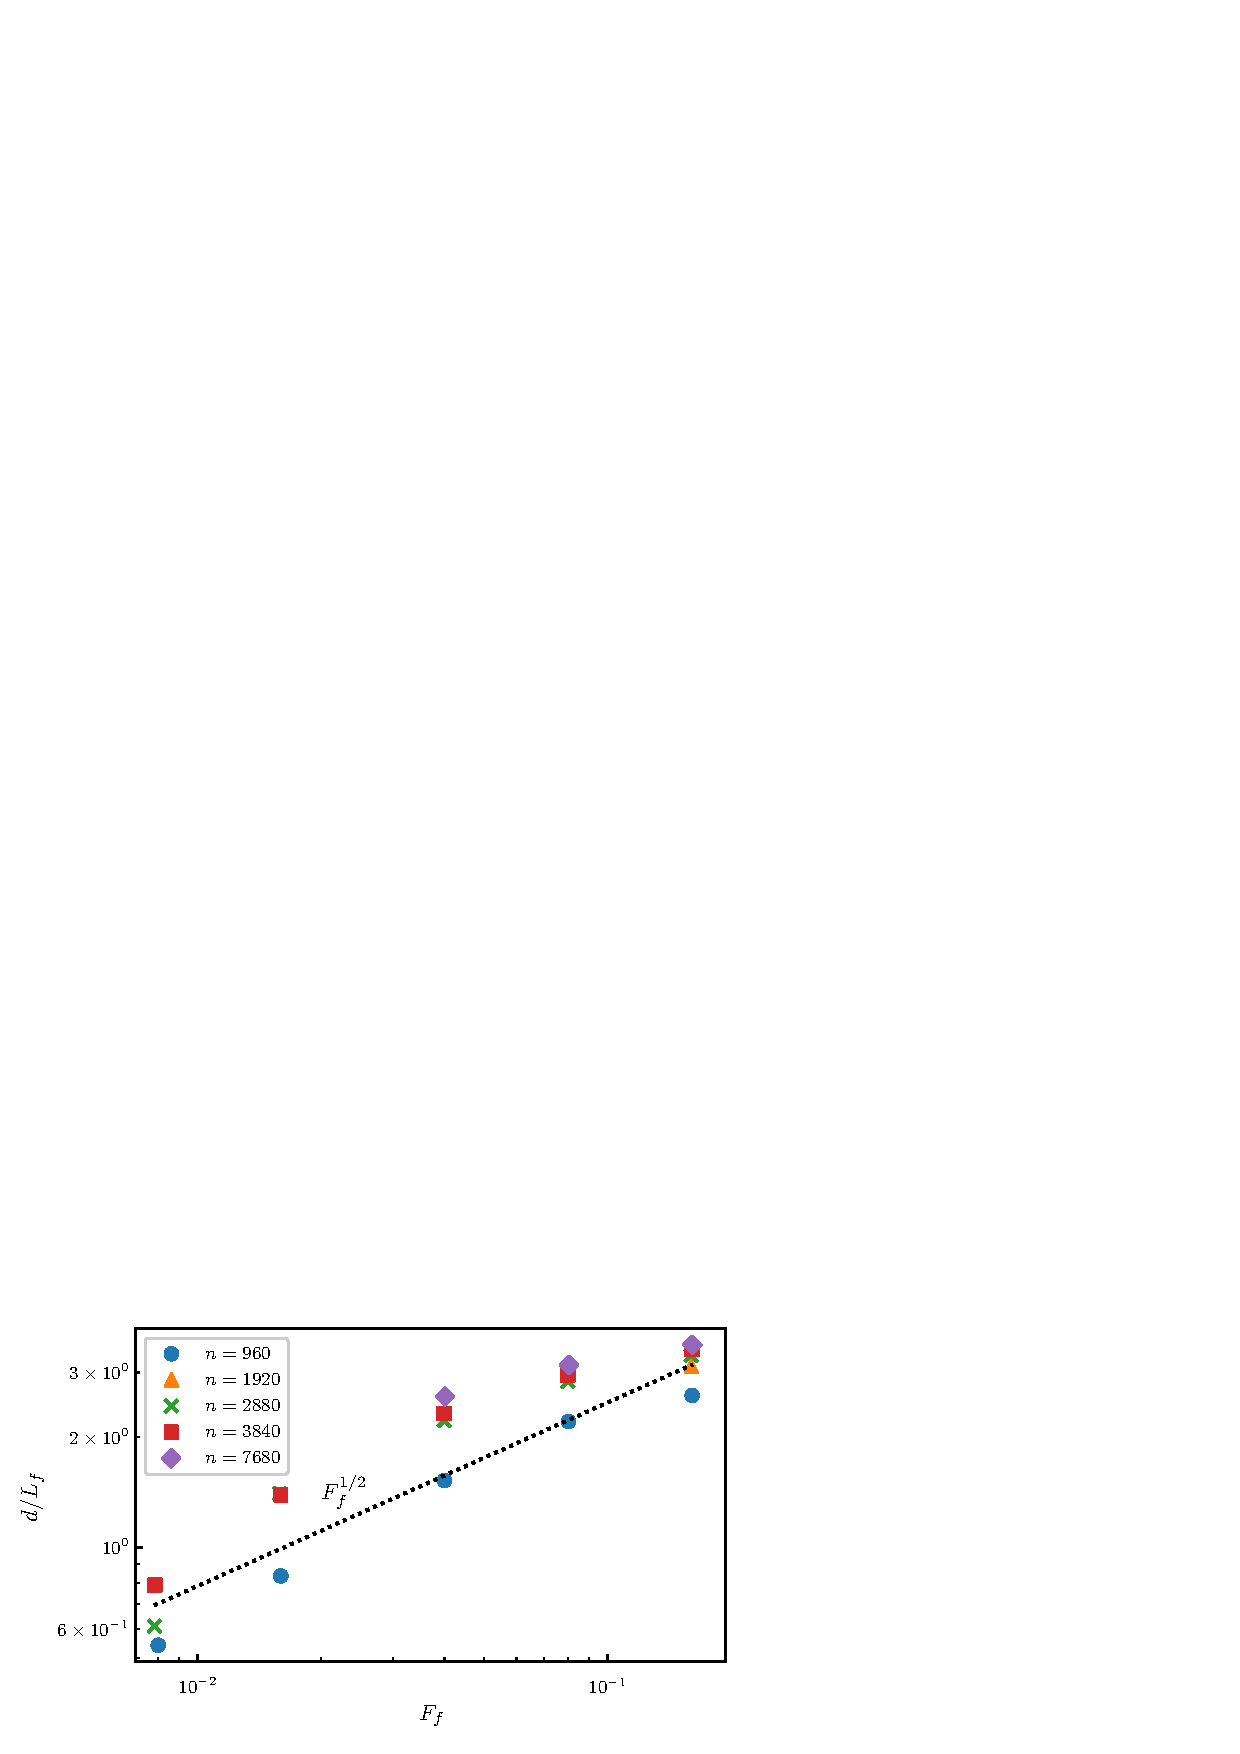
\includegraphics[width=9cm]{paper_04_shallow_water/Pyfig/fig13}}
\caption{Mean distance between the shocks as function of Froude number.  }
\label{fig_distance_lap}
\end{figure}


\begin{figure}
\centerline{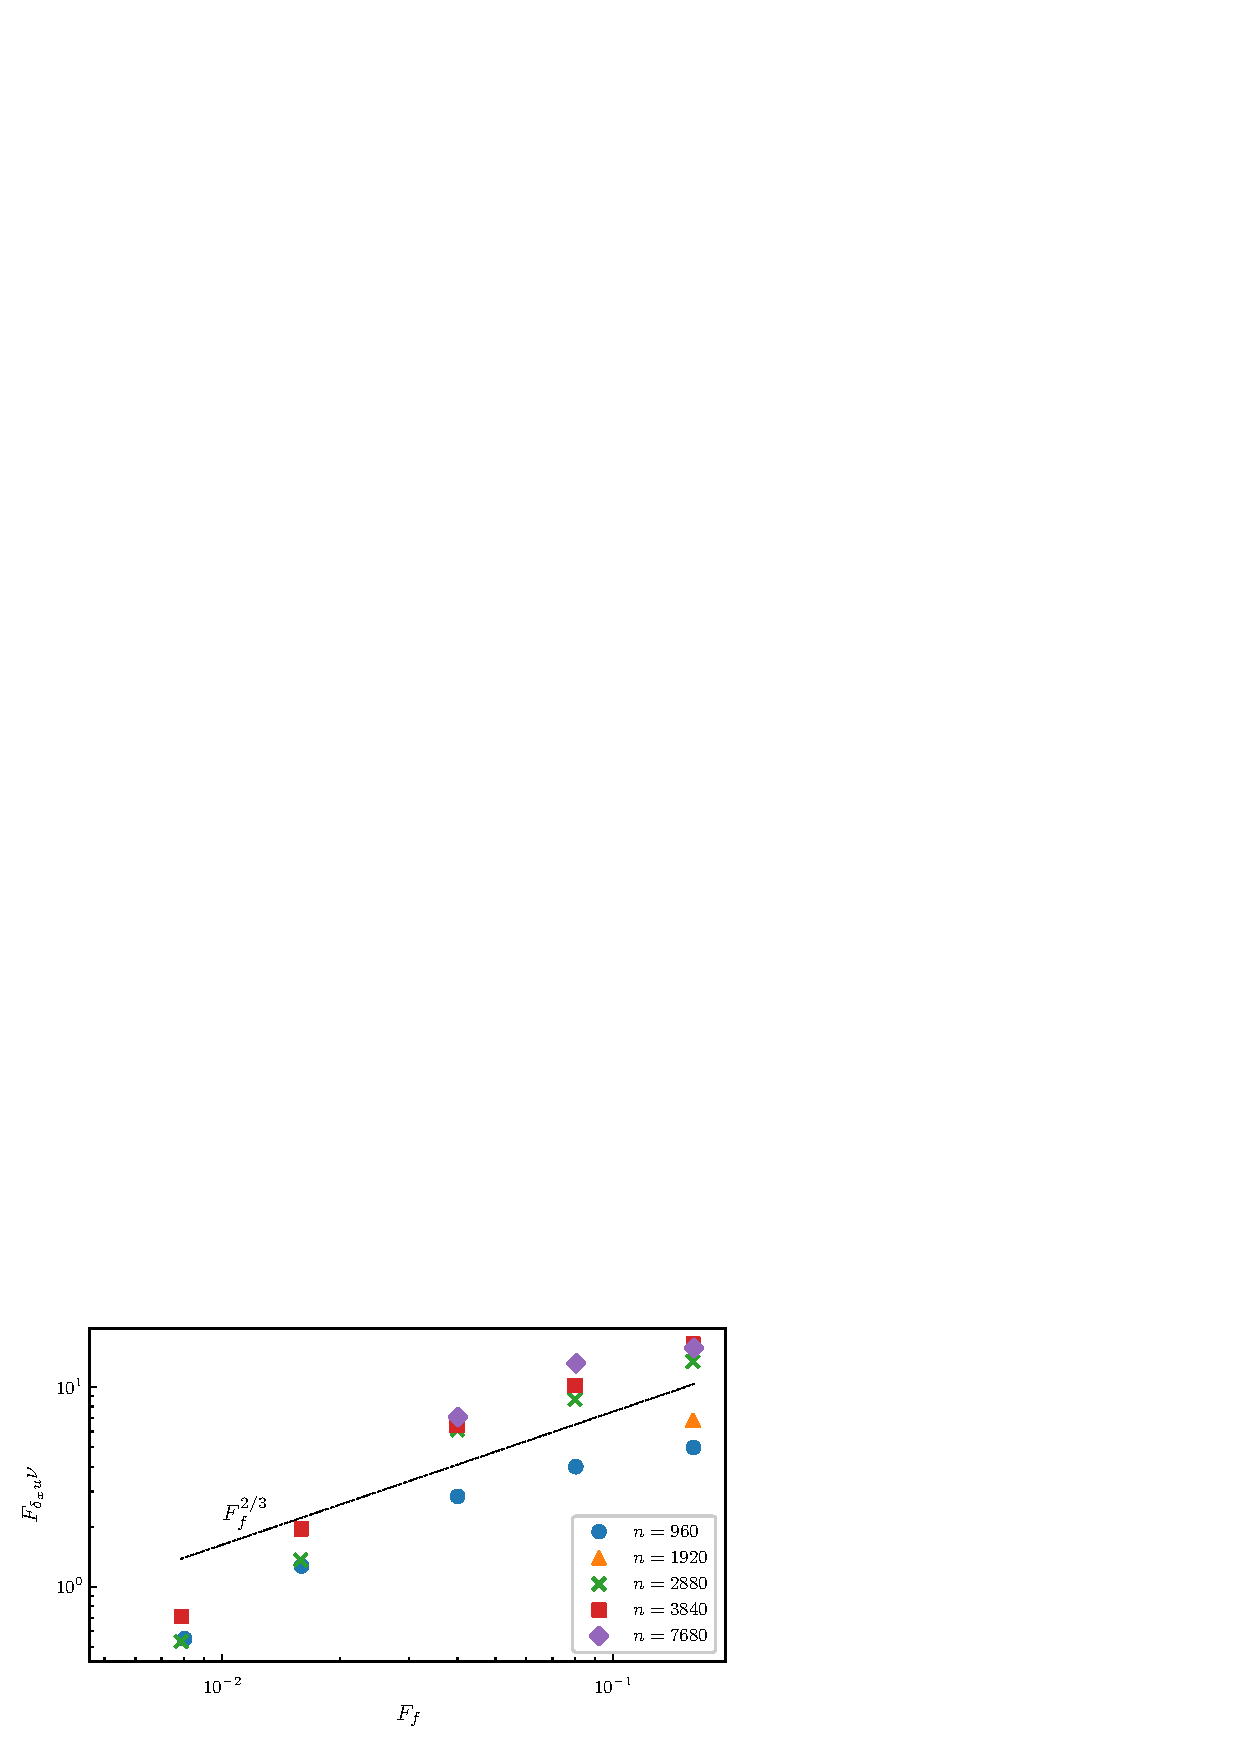
\includegraphics[width=9cm]{paper_04_shallow_water/Pyfig/fig14}}
\caption{Flatness of divergence $ \nabla \cdot {\bf u} $ times viscosity $ \nu $, versus $ F_f $. Dotted straight line indicates $ F_f^{2/3} $. }
\label{FlatnessDiv}
\end{figure}

\begin{figure}
\centerline{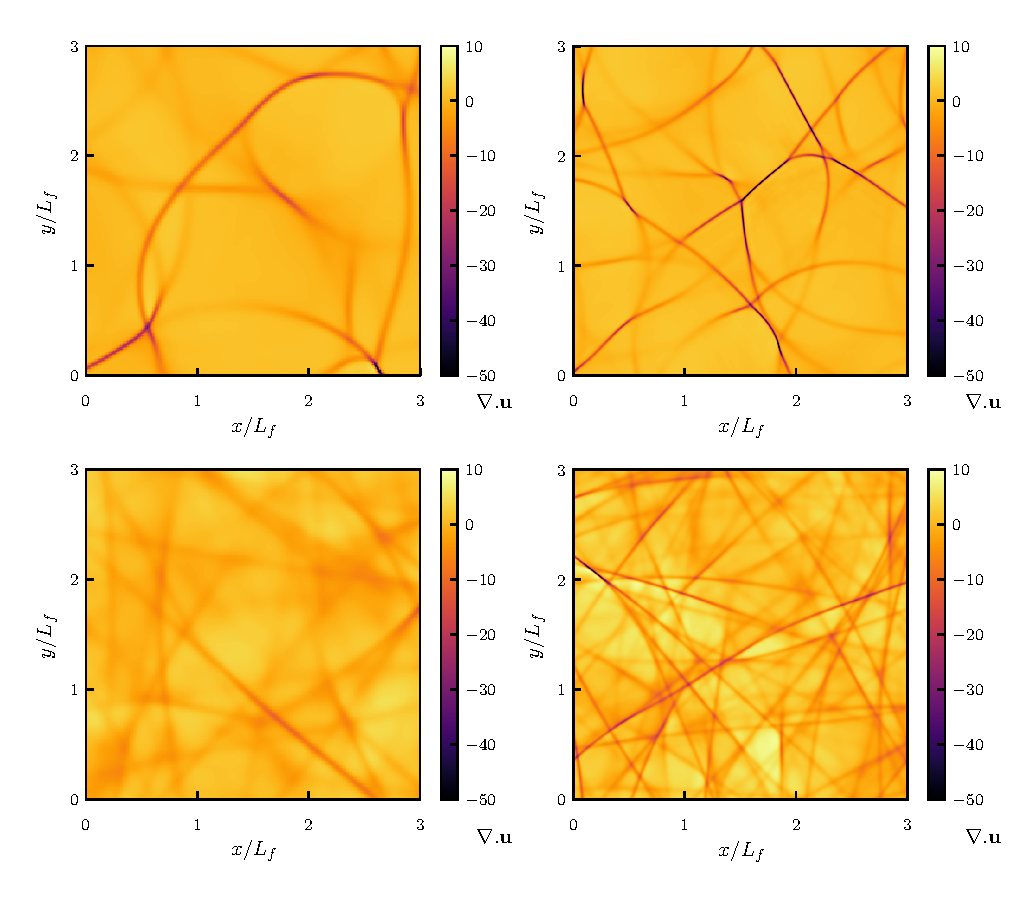
\includegraphics[]{paper_04_shallow_water/Pyfig/fig15}}
\caption{$ \nabla \cdot {\bf u} $ for four different runs. Upper left: WL1, $ Re = 68 $, $ F_f = 0.16 $; Upper right:  { WL3,  $ Re = 203 $, $ F_f = 0.16 $;} Lower left: WL17, $ Re = 68 $, $ F_f = 0.008 $; Lower right: WL18,  $ Re = 199 $, $ F_f = 0.008 $.}
\label{Physical_lap}
\end{figure}




The dynamics of the runs with Laplacian diffusion was similar to the runs with higher-order diffusion. In figure \ref{MeanE2} we see mean energy in the stationary state versus $ c $ to the left and versus $ n $ to the right.
The variation of mean energy with $ c $ seems to be a little bit weaker for these runs as compared to the runs with hyper diffusion.  { However, the higher resolution runs are relatively close to approaching the $ c^{1/2} $-scaling.}
The variation of mean energy with resolution, or Reynolds number, is quite similar to what is seen in the corresponding plot \ref{MeanE}. For each $ c $ there is a monotonic increase of mean energy with resolution, and the increase is becoming stronger as $ c $ is increased, with comparable but not equal values of the exponent $ \alpha $.


In figure \ref{fig_distance_lap} we see the mean distance between the shocks as a function of $ F_f $, together with a straight line indicating $ F_f^{1/2} $. { As compared to the runs with hyperviscosity there is a larger spread of the points and the $ F_f^{1/2} $ scaling is not as clear. The lower Reynolds number series ($ Re \approx 70 $ blue dots) falls below the higher Reynolds number series. This may be explained by the fact that the shock detection algorithm is much more sensitive to the threshold value which is used for $ \nabla \cdot {\bf u} $ in these simulations than in the simulations with hyperviscosity.  In particular, this is true in the lower Reynolds number runs. } In figure \ref{FlatnessDiv} we see the flatness of the divergence, multiplied by $ \nu $, versus $ F_f $. According to (\ref{FD}) we should have $ F_{\partial u} \nu \propto  d^{4/3} $ and if $ d \propto Fr^{1/2} $, the points should collapse on a single line, $ F_f^{2/3} $.  {For the three largest $ F_f $, there is a relatively good collapse of the points from the three highest  Reynolds numbers series, supporting both the $ \nu^{-1} $-scaling and the $ F_f^{2/3} $-scaling. }
 The lower Reynolds number runs (blue dots) fall below the higher Reynolds number runs, which we interpret as a low Reynolds number effect. The points corresponding to the two lowest values of $ F_f $ fall below the prediction $ F_f^{2/3} $. This can be explained by the fact that the shocks are on the verge of fading away in these runs. Clearly, a necessary condition for shocks to be present is that the mean distance between them is much larger than their  width, that is
\begin{equation} \label{Condition}
\frac{d}{\delta x} \gg  1\, .
\end{equation}
Since $ F_{\partial u} \propto d/\delta x $, this means that the flatness of divergence must be much larger than unity. Substituting (\ref{Width}) into (\ref{Condition})  and assuming that (\ref{MeanDistance}) is valid we can formulate the condition as
\begin{equation}  \label{SCond}
Re F_f^{2/3} \gg 1 \, .
\end{equation}
If this condition is not fulfilled the shocks will fade away.  In figure
\ref{Physical_lap} we have plotted the divergence for four different runs with
different $ Re $ and $ F_f $. It should be pointed out again, that the area of
the computational domain is sixteen times larger than area of the outcuts shown
in the figures.  $(a,b)$ are from simulations with  $ F_f = 0.16 $ but
different $ Re $ ($ Re = 68\, (a) $ and { $ Re = 203\, (b) $ }).
As can be seen, the shocks are wider in the lower Reynolds number run $(a)$
than in the higher Reynolds number run $(b)$, as expected. $(c)$
is from a simulation with the same $ Re $ as in $(a)$, but with a much smaller
$ F_f $. In this simulation we have $ Re F_f^{2/3} = 2.7 $, so the condition
(\ref{SCond}) is not fulfilled, and the
shocks have almost faded away. $(d)$ is from a simulation with
the same $ F_f $ as in $(c)$, but with a higher $ Re = 199 $.
Here, $ Re F_f^{2/3} = 7.8 $ and  the shocks are clearly discernible. {
Comparing $(b)$ and $(d)$ with each other, they have approximately the same
$ Re $, while the lower one has a considerably lower $ F_f $.  In this run the
shocks are denser and straighter as compared to the higher $ F_f $-run.}



% \bibliographystyle{jfm}
% \bibliography{biblio}
%
% \end{document}
